% !TeX program = xelatex
% 编译: latexmk -xelatex main.tex  (或 xelatex main.tex 两次 + bibtex)
\documentclass[12pt,a4paper]{ctexart}

\usepackage{amsmath,amssymb,bm}
\usepackage{graphicx}
\usepackage{float}
\usepackage{booktabs}
\usepackage{tabularx}
\usepackage{longtable}
\usepackage{geometry}
\usepackage[table]{xcolor}
\usepackage{tcolorbox}
\tcbuselibrary{breakable,skins}
\usepackage{enumitem}
\usepackage{caption}
\usepackage{hyperref}

\geometry{margin=1.3cm}
\linespread{1.12}
\graphicspath{{figures/}}
\captionsetup{font=small,labelfont=bf}
\hypersetup{colorlinks=true,linkcolor=blue!60!black,citecolor=green!50!black,
            urlcolor=blue!60!black}

% ---- 常用记号 ----
\newcommand{\dd}{\mathrm{d}}
\newcommand{\jj}{\mathrm{j}}
\newcommand{\bx}{\bm{x}}
\newcommand{\bu}{\bm{u}}
\newcommand{\bA}{\bm{A}}
\newcommand{\bB}{\bm{B}}
\newcommand{\bY}{\bm{Y}}
\newcommand{\bG}{\bm{G}}
\newcommand{\bT}{\bm{T}}
\newcommand{\bz}{\bm{z}}
\newcommand{\bV}{\bm{V}}
\newcommand{\bI}{\bm{I}}
\newcommand{\bzero}{\bm{0}}
\newcommand{\Real}{\operatorname{Re}}
\newcommand{\Imag}{\operatorname{Im}}
\newcommand{\pu}{\mathrm{p.u.}}
\newcommand{\trans}[1]{{#1}^{\!\top}}
\newcommand{\dif}[2]{\frac{\dd #1}{\dd #2}}
\DeclareMathOperator{\diag}{diag}
\DeclareMathOperator{\rank}{rank}

% ---- 推导块盒子 ----
\newtcolorbox{derivblock}[1]{
  breakable, enhanced,
  colback=blue!3!white, colframe=blue!45!black,
  boxrule=0.7pt, arc=2pt,
  left=5pt, right=5pt, top=4pt, bottom=4pt,
  coltitle=white, colbacktitle=blue!45!black,
  title={#1}, fonttitle=\bfseries\small,
  attach boxed title to top left={xshift=6pt, yshift=-\tcboxedtitleheight/2},
  boxed title style={size=small, colframe=blue!45!black}
}

\title{\bfseries 电网多尺度建模：三类模型的连接与 Kuramoto 模型\\[4pt]
\large 第一次讨论·子任务 3 的调研}
\author{电网承载力评估与优化技术研究项目组}
\date{2026 年 9 月}

\begin{document}
\maketitle

\begin{abstract}
本报告对应第一次讨论分工中的第 3 项任务：“EMT（仅需了解）与多尺度建模（重要）”。
报告以四个问题组织：\textbf{Q1} 什么是 EMT、为什么它不可替代但在本项目中大概率不作为主线；
\textbf{Q2} 潮流（PF/QSTS）、RMS、EMT 三类模型的假设、忽略的物理过程、时间尺度与状态变量；
\textbf{Q3} 潮流与 RMS 之间如何连接、交换什么变量（多尺度降阶与混合仿真接口）；
\textbf{Q4} Kuramoto 模型为什么能刻画电网、其假设与变量含义、以及与 RMS 模型的关系。
每个结论都配以可复现的数值图（\texttt{python/} 下脚本，\texttt{figures/} 下矢量图）
与关键推导，便于核查与讨论。在方法上，本报告把三类模型统一为同一多尺度系统的
三种降阶水平，从而把“模型连接”问题归结为跨尺度降阶的保真度问题。
\end{abstract}

\tableofcontents
\vspace{1em}

\section{任务、问题与记号约定}
\label{sec:intro}

\subsection{本报告要回答的问题}

第一次讨论对本部分的原文要求是：

\begin{quote}\itshape
3. EMT（仅需了解，后续大概率不会用到）与多尺度建模（重要）。
EMT 模型最复杂，简单科普一下 EMT 即可。需要调研电网的多尺度建模：先了解
潮流/RMS/EMT 这 3 类模型的假设是什么、忽略了哪些物理过程、研究哪个时间尺度、
有哪些变量；然后调研潮流和 RMS 模型之间怎么连接、之间传什么变量等。
Kuramoto 模型为什么可以用来研究电网，用 Kuramoto 模型研究电网假设是什么、
并解释变量含义、Kuramoto 模型与 RMS 模型有什么关系。
\end{quote}

据此把任务拆成四个可以独立回答、也可以被逐条质疑的问题：

\begin{description}[leftmargin=2.2em]
\item[Q1（EMT 简介）] 什么是电磁暂态（EMT）模型？它保留了什么别的模型丢弃的物理过程？
为什么它不可替代，但在本项目中不作为主线？
\item[Q2（三类模型对照）] 潮流（PF/QSTS）、RMS、EMT 各自的数学形式、假设、
忽略的物理过程、时间尺度、状态变量是什么？三者之间是“不同精度的同一模型”，
还是“不同假设下的不同模型”？
\item[Q3（多尺度连接，重点）] 潮流与 RMS 之间如何连接、传什么变量？
为什么可以把完整模型降阶为相量模型，误差有多大？混合 EMT--RMS 仿真的接口
交换什么、代价是什么？
\item[Q4（Kuramoto，重点）] 为什么 Kuramoto 振子模型能研究电网？
它做了哪些假设、变量对应什么物理量？它与 RMS 模型是等价、近似还是降阶？
\end{description}

\subsection{记号与核心概念约定}
\label{sec:notation}

为了避免“同一个词在不同章节指不同东西”，先固定本报告的用法。
每个定义都给出\textbf{为什么需要它}，后文首次使用时不再重复解释。

\begin{description}[leftmargin=2.4em]
\item[模型] 指“一组方程 $+$ 一组假设 $+$ 一个适用范围”。因此说“EMT 模型”时，
同时意味着它的假设（保留全部 $L,C$ 动态、可含开关）和适用范围（$\mu$s--ms）。
本报告中“三类模型”始终指 PF/QSTS、RMS、EMT。
\item[状态变量] 指真正带时间导数、需要初值的量（记 $\bx$）；
与之相对的是由代数约束即时确定的量（记 $\bm{y}$，如潮流中的 $V,\theta$）。
区分二者是理解“PF 没有状态、RMS 有状态”的关键。
\item[平衡点（工作点）] 令所有时间导数为零后方程的解。潮流解就是
RMS 方程~\eqref{eq:rms-dae} 的平衡点；这是 \S\ref{sec:workpoint} 的第一层连接。
\item[相量] 把一个窄带正弦信号 $a(t)=A(t)\cos(\omega_s t+\varphi(t))$
的幅值与相位打包为复数 $\underline{A}=A e^{\jmath\varphi}$
（用 $A$ 而非有效值时也称“峰值相量”）。
相量成立的前提是 $A(t),\varphi(t)$ 相对载波（此处指 $50$ Hz 工频正弦）变化足够慢——这个“足够慢”
在 \S\ref{sec:quasi} 被量化为一个不等式。
\textbf{相量不是某一类模型专属}：PF 与 RMS 都用它，区别在于\textbf{相量是否随时间变化}——
PF 中相量取常数（因此是代数方程），RMS 中相量是随时间慢变的复包络（因此是微分方程）；
EMT 不用相量，直接求瞬时值。
\item[降阶] 在\textbf{关注的时间尺度上}保持所需精度的前提下，用更少的状态或更弱的方程替代原系统；
降阶的代价是丢掉该尺度之外的动态与非线性细节（因此“潮流丢掉全部动态”与“Kuramoto 保留相角动态”
都是合法的降阶，只是关注点不同）。本报告的三类模型与 Kuramoto 正处在这样一个简化关系之中（式~\eqref{eq:chain}）。
\item[时间尺度分离] 存在小参数 $0<\varepsilon\ll1$，使系统可写成
$\dot\bx=\bm f(\bx,\bz),\ \varepsilon\dot\bz=\bm g(\bx,\bz)$（$\bx$ 为慢变量、$\bz$ 为快变量）。
它使“忽略快变量”从经验做法变成有误差界可言的数学操作（\S\ref{sec:singular}）。
\item[多尺度建模] 指在同一研究目标下\textbf{同时或交替}使用不同尺度的模型，
并且\textbf{显式定义}它们之间交换什么变量、以什么步长、误差多大
（\S\ref{sec:q3} 的三层连接）。
\end{description}

\subsection{与项目书技术点的对应}

本部分对应项目书技术内容第一点“基于时空动力学的分布式资源高维非线性接入行为建模技术”，
以及技术难点第二点“多源外部不确定因素对电网运行影响难以准确刻画”，
并为技术内容第二点（有限元/伽辽金改进潮流计算）提供“哪些动态可以安全忽略”
的判据依据：只有先说清各模型忽略了什么，才能判断在什么条件下可以安全地降阶与加速。

\subsection{阅读路线}

若时间有限，只读三处即可覆盖全部结论：表~\ref{tab:retention}（三模型保留矩阵）、图~\ref{fig:chain}（模型之间的简化关系）、表~\ref{tab:assumptions}（每条结论的假设与失效条件）。
如需查阅具体步骤与公式，见正文的 6 个推导块（【推导块 1--6】，分别位于 \S\ref{sec:q3}、\S\ref{sec:q4}）；
符号与缩略语分别见附录~\ref{app:symbols}、附录~\ref{app:abbr}，设备与概念释义见附录~\ref{app:concepts}。

\section{Q1：EMT 是什么，以及它在项目中的定位}
\label{sec:q1}

\noindent\textbf{本章回答}：EMT 是什么、保留了哪些动态、为什么本项目不以它为主线。
组织顺序是：先说明它为什么必要（快动态进来了），再给方程与保留清单，最后交代代价与定位。

\subsection{物理动机：电力电子化把“快”带进了电网}

“电力电子化”指电网中通过变流器接入的电源与负荷（光伏、风电、储能、电动汽车、直流输电）
占比不断提高，其特征是\textbf{控制动作快、系统惯量低}。
传统输电网的动态由同步机主导：惯性时间常数 $H=2\text{--}9$ s，
机电振荡频率 $0.1\text{--}2$ Hz，一次调频时间常数数秒到数十秒。
在这种系统里，电压电流在 50 Hz 附近是窄带信号，用“幅值$+$相角”的
相量（phasor）描述就足够，网络可以用代数方程表示。

分布式资源大规模接入后，电网里多了另一类元件：由 IGBT/SiC 构成的电压源型变流器（VSC）。
它们的开关频率 $f_{sw}$ 通常在 $2\text{--}20$ kHz（SiC 可达上百 kHz），
内环电流控制带宽约 $0.5\text{--}2$ kHz，PLL 带宽约 $50\text{--}500$ Hz。
这些动态的时间常数在 $10^{-6}\text{--}10^{-2}$ s，已经接近甚至快于 50 Hz 载波周期
$T_0=20$ ms。此时“相量”假设的前提（信号窄带、网络瞬间建立）不再成立，必须直接求解
三相瞬时值，这就是电磁暂态（Electromagnetic Transient, EMT）模型。

图~\ref{fig:timescales} 把这一事实量化：同一套电网的研究对象从
$1\,\mu$s（开关、行波）一直延伸到 $10^{9}$ s（约 32 年，规划），
跨度约 15 个数量级；三类模型各自覆盖其中一段，且相邻两段只在边界处重叠。

\begin{figure}[htbp]
\centering
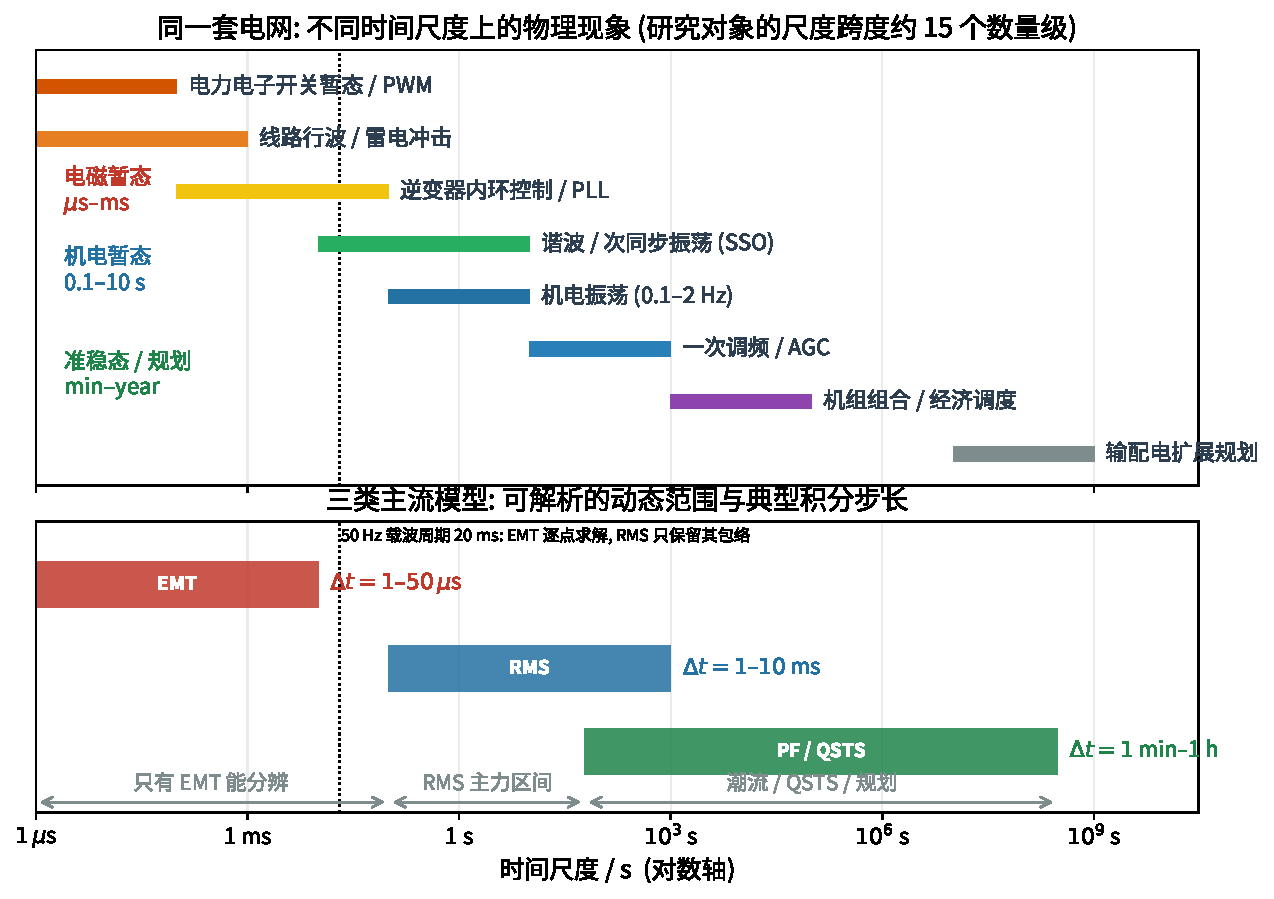
\includegraphics[width=0.99\textwidth]{fig01_model_timescales.pdf}
\caption{\textbf{这张图说明}：电网里的事快慢相差约十五个数量级，不可能用一个模型同时覆盖。
\textbf{看图}：横轴为对数时间尺度；上半部分彩色横条是各物理现象所在的尺度区间，
下半部分三条色带为三类模型的适用范围与典型步长；竖直虚线为 50 Hz 周期（20 ms）。
\textbf{结论}：三类模型不是精度之争，而是研究对象不在同一时间尺度。}
\label{fig:timescales}
\end{figure}

\subsection{EMT 的建模对象与方程}

EMT 在 $abc$（或 $\alpha\beta0$）坐标下直接离散元件方程。
最基础的三个元件是
\begin{equation}
\underbrace{v_R = R\,i_R}_{\text{电阻（代数）}},\qquad
\underbrace{v_L = L\,\dif{i_L}{t}}_{\text{电感（微分）}},\qquad
\underbrace{i_C = C\,\dif{v_C}{t}}_{\text{电容（微分）}} .
\label{eq:emt-elements}
\end{equation}
\textbf{读法}：三个元件中只有电阻是代数关系，电感与电容各含一个时间导数——
这正是 EMT 与稳态模型的根本区别：EMT 必须保留这两个导数。

把每个元件写成式~\eqref{eq:emt-elements} 后，对每个电气节点列基尔霍夫电流定律（KCL），
得到一组关于瞬时量的微分--代数方程
\begin{equation}
\begin{cases}
\dot{\bx} = \bm{f}(\bx,\bm{y},\bu,t),\\[2pt]
\bzero = \bm{g}(\bx,\bm{y},\bu,t),
\end{cases}
\qquad
\bx\in\mathbb{R}^{n},\ \bm{y}\in\mathbb{R}^{p},\ \bu\in\mathbb{R}^{m}.
\label{eq:emt-dae}
\end{equation}
其中 $\bx$ 为状态变量（需初值、随时间演化，如线路电感电流、节点电容电压），
$\bm{y}$ 为代数变量（由约束即时确定，主要是各节点电压），
$\bu$ 为\textbf{输入/控制变量}（例如机组的机械功率 $P_m$、励磁电压、变流器的功率指令），
$t$ 为时间。与 RMS 的差别在于：EMT 的 $\bx$ 里\textbf{包含全部网络贮能元件}（因此 $n$ 很大），
$\bm{f}$ 中的开关函数使方程分段连续，$\bm{g}$ 中的约束来自纯电阻连接与理想电源。
\textbf{读法}：$\bm{f}$ 描述“怎么变化”，$\bm{g}$ 描述“每时刻必须满足的约束”；
EMT 的状态维数 $n$ 很大，且步长小、步数多——三者共同造成其计算量远高于潮流/RMS。

长线与电缆需用分布参数（行波）模型而非集中参数；
\textbf{这也解释了为什么只有 EMT 能算雷电冲击与行波}——相量模型假设网络“瞬时建立”
（把行波时间视为零），做不到这一点。

\begin{table}[htbp]
\centering
\small
\renewcommand{\arraystretch}{1.15}
\begin{tabular}{@{}lccc@{}}
\toprule
物理过程 & PF/QSTS & RMS & EMT \\
\midrule
网络 KCL/KVL（瞬时） & \cellcolor{yellow!40}$\approx$ & \cellcolor{yellow!40}$\approx$ & \cellcolor{green!25}$\surd$ \\
网络 $L,C$ 电磁暂态 & \cellcolor{red!15}$\times$ & \cellcolor{red!15}$\times$ & \cellcolor{green!25}$\surd$ \\
分布参数 / 行波传播 & \cellcolor{red!15}$\times$ & \cellcolor{red!15}$\times$ & \cellcolor{green!25}$\surd$ \\
同步机定子磁链动态（快） & \cellcolor{red!15}$\times$ & \cellcolor{red!15}$\times$ & \cellcolor{green!25}$\surd$ \\
转子摇摆动态（慢） & \cellcolor{red!15}$\times$ & \cellcolor{green!25}$\surd$ & \cellcolor{green!25}$\surd$ \\
调速器 / 原动机动态 & \cellcolor{red!15}$\times$ & \cellcolor{yellow!40}$\approx$ & \cellcolor{green!25}$\surd$ \\
励磁 / AVR 动态 & \cellcolor{red!15}$\times$ & \cellcolor{yellow!40}$\approx$ & \cellcolor{green!25}$\surd$ \\
变流器 PWM 开关过程 & \cellcolor{red!15}$\times$ & \cellcolor{red!15}$\times$ & \cellcolor{green!25}$\surd$ \\
逆变器内环电流控制 & \cellcolor{red!15}$\times$ & \cellcolor{yellow!40}$\approx$ & \cellcolor{green!25}$\surd$ \\
PLL / 外环控制 & \cellcolor{red!15}$\times$ & \cellcolor{yellow!40}$\approx$ & \cellcolor{green!25}$\surd$ \\
三相不平衡与负序/零序 & \cellcolor{yellow!40}$\approx$ & \cellcolor{yellow!40}$\approx$ & \cellcolor{green!25}$\surd$ \\
非额定频率下的偏离 & \cellcolor{red!15}$\times$ & \cellcolor{yellow!40}$\approx$ & \cellcolor{green!25}$\surd$ \\
全阶微分方程（未降阶） & \cellcolor{red!15}$\times$ & \cellcolor{yellow!40}$\approx$ & \cellcolor{green!25}$\surd$ \\
\bottomrule
\end{tabular}
\caption{三类模型对物理过程的保留程度。$\surd$ 完整保留，
$\approx$ 准稳态/平均/参数化，$\times$ 忽略或退化为代数约束。
\textbf{图的目的}：把“三模型差异”从定性说法变成逐条可核对的清单；
例如“变流器 PWM 开关过程”一行，只有 EMT 是 $\surd$，这正是
式~\eqref{eq:emt-dae} 中开关函数的作用。}
\label{tab:retention}
\end{table}

\subsection{EMT 的求解与步长（定性）}

EMT 的方程用\textbf{隐式积分}逐步推进（工程上最常用梯形法\cite{dommel1969,watson2007}；
国内电磁暂态仿真技术的系统综述见文献\cite{dong2018}）。
它的计算结构与潮流/RMS 有本质区别：把电感、电容在每个时步等值为
“电导 $+$ 历史电流源”（诺顿等值），因此\textbf{每个时步只需解一次线性方程组}，
而不是像潮流那样解非线性方程并做牛顿迭代。这解释了“EMT 步数多但每步便宜、
潮流步数少但每步贵”的差别。

步长由\textbf{最高关心频率} $f_{\max}$ 决定（开关频率、网络谐振、$LC$ 振荡中最大者）：

\begin{equation}
\Delta t \;\lesssim\; \frac{1}{10\sim20\,f_{\max}} .
\label{eq:emt-dt}
\end{equation}
\textbf{读法}：步长与最高关心频率成反比——想看得越快，步长就必须越小；这就是“分辨率”的直接体现。

对 $10$ kHz 开关的变流器，$\Delta t\lesssim5\,\mu$s；工程上取 $1$--$50\,\mu$s
（图~\ref{fig:timescales}）。一次秒级仿真因此需要 $10^{5}$--$10^{6}$ 步，
这是 EMT 计算量远高于潮流/RMS 的直接原因（刚度比的定量讨论见 \S\ref{sec:eigen}）。
其数值细节（梯形法推导、伴随电路、临界阻尼调整、开关插值）不在本报告展开。

\subsection{EMT 在本项目中的定位}

本项目要回答的是“城市电网还能接入多少分布式资源”，其评估与优化尺度为
分钟--小时--年（图~\ref{fig:timescales} 下半的 PF/QSTS 段），
对应的模型是潮流与准稳态时序模型。引入 EMT 不会改变承载力指标的定义，
只会把计算量提高 $10^{3}\text{--}10^{6}$ 倍（见 \S\ref{sec:eigen} 的刚度比）。
因此 EMT 在本项目中的定位是：
\begin{enumerate}[leftmargin=1.6em]
\item \textbf{判据提供者}：给出“哪些动态可以安全忽略”的边界（\S\ref{sec:quasi}、\S\ref{sec:singular}）；
\item \textbf{局部验证器}：对高比例 IBR 的薄弱片区做详细校验，而不是全网主算；
\item \textbf{解释素材}：解释为什么 RMS/相量模型在电力电子化下会失效。
\end{enumerate}

\paragraph{小问题 1：EMT 既然用不到，为什么还要调研？}
除了上面三条，还有一个直接原因：本项目技术内容第二点要“改进潮流计算”，
而改进的前提是知道\textbf{潮流到底忽略了什么、在什么条件下可以忽略}。
式~\eqref{eq:qs-error} 与式~\eqref{eq:eps-grid} 就是这条判据的量化形式；
没有 EMT 这一端，判据无从谈起。

\paragraph{小问题 2：“暂态”和“稳态”怎么区分？}
本报告统一用\textbf{时间尺度}而不是“时间长短”来定义：
若某变量的时间常数 $\tau_x$ 与关注现象的时间尺度相当，它就是“动态的”（暂态问题）；
若 $\tau_x$ 远小于关注尺度，则它在该尺度上“瞬时建立”，可用代数约束替代（稳态问题）。
这样定义的好处是：同一个电感在 EMT 中是动态的、在潮流中是代数的，
差别只来自关注尺度不同——这正是表~\ref{tab:retention} 中
“网络 $L,C$ 电磁暂态”一行从 EMT 的 $\surd$ 变为 PF 的 $\times$ 的含义。

这与讨论中的判断一致：EMT“仅需了解，后续大概率不会用到”，但多尺度建模“重要”。

\section{Q2：PF/QSTS、RMS、EMT 三类模型的对照}
\label{sec:q2}

\noindent\textbf{本章范围}：只做\textbf{对照}——三类模型各自的假设、忽略的物理过程、
时间尺度与状态变量，这是本部分任务明确要求的内容。
潮流（含 AC/配电网/三相潮流、DistFlow、QSTS、DER 接入后的变化）与
RMS 的建模细节分别是第 1、2 项任务的调研内容，本章只引用其结论，不重复推导。

\subsection{三类模型的形式与变量}

\paragraph{潮流 / QSTS（主线模型）。}
假设：稳态、单一频率、输电网三相平衡。节点功率平衡方程为\cite{kundur1994,sauer1998}
\begin{equation}
P_i=V_i\sum_{k=1}^{n}V_k\bigl(G_{ik}\cos\theta_{ik}+B_{ik}\sin\theta_{ik}\bigr),\qquad
Q_i=V_i\sum_{k=1}^{n}V_k\bigl(G_{ik}\sin\theta_{ik}-B_{ik}\cos\theta_{ik}\bigr),
\label{eq:power-flow}
\end{equation}
待求量为各节点电压幅值与相角 $(V_i,\theta_i)$，\textbf{没有状态变量}。
\textbf{读法}：这是一组\textbf{纯代数方程}——未知量只有各节点的电压幅值与相角；
式中的 $G_{ik},B_{ik}$ 来自网络导纳，$\theta_{ik}=\theta_i-\theta_k$ 是相角差。
式~\eqref{eq:power-flow} 的完整推导（KCL $\to$ 节点导纳 $\to$ 复功率 $\to$ 功率方程）
见附录~\ref{app:powerflow}，属第 1 项任务的调研范围，正文只引用结论。
式~\eqref{eq:power-flow} 中\textbf{没有任何时间导数}——这不是因为它“静态”，
而是所有时间导数项都被假设为零：在 \S\ref{sec:singular} 会证明，
令 RMS 的微分--代数方程所有导数 $=0$，得到的正是式~\eqref{eq:power-flow}。
把负荷与 DER 的时序逐点代入求解，即\textbf{准稳态时序模型（QSTS）}，
它是承载力评估最常用的计算内核\cite{dlt2041,ge2023}。

\paragraph{RMS（机电暂态/相量域动态）。}
假设有两条：
（i）网络的时间常数（毫秒级）远小于所关心的机电动态（秒级），
因此每一时刻网络都可以用代数方程表示，不必描述其暂态过程；
（ii）三相近似对称，可用\textbf{正序相量}——把一组对称的三相量合成为一个等效单相量——来描述运行状态。
其形式为微分--代数方程\cite{machowski2020,milano2010}
\begin{equation}
\dot{\bx}=\bm{f}(\bx,\bm{y},\bu),\qquad
\bzero=\bm{g}(\bx,\bm{y},\bu),
\label{eq:rms-dae}
\end{equation}
其中
\begin{itemize}[leftmargin=1.6em]
\item $\bx$：真正带时间导数的\textbf{状态}——转子角 $\delta$、转速 $\omega$、暂态电势
$E_q'$，以及调速器/励磁/稳定器与变流器外环、PLL 等控制器状态；
\item $\bm{y}$：瞬时建立、由代数约束确定的量——节点电压 $(V,\theta)$，
即式~\eqref{eq:power-flow} 的复数形式。
\end{itemize}
\textbf{读法}：第一式描述“状态怎么随时间变化”（微分方程），
第二式描述“每一时刻必须满足的网络约束”（代数方程）；
两者必须联立求解，这也是“微分--代数方程（DAE）”这一名称的来源。
DER 如何加入（GFL/GFM、聚合模型\cite{hang2021}）与数值求解方法，
属第 2 项任务的调研内容，本章不展开。

\paragraph{EMT（电磁暂态）。}
见 \S\ref{sec:q1}：$abc/\alpha\beta0$ 瞬时域、保留网络贮能元件与开关动态，
步长 $1\text{--}50\,\mu$s。

\subsection{三者对照}

表~\ref{tab:models} 汇总差异。有三点需要强调：
\begin{enumerate}[leftmargin=1.6em]
\item \textbf{“正序/三相”与“相量/瞬时”是两个正交的维度。}
配电网潮流（DistFlow、三相不平衡 PF）可以是“三相 $+$ 稳态”（仍属 PF 族）；
RMS 通常是“正序 $+$ 动态”；EMT 是“三相 $+$ 瞬时”。
\item \textbf{时间尺度不是模型本身，而是模型的分辨率。}
三类模型描述的是\textbf{同一个物理系统}，只是保留的动力学阶数不同；
因此在 \S\ref{sec:q3} 可以把它们写成同一条降阶链条。
\item \textbf{“忽略”不等于“不存在”。}
RMS 忽略网络电磁暂态，等价于承认网络“瞬时建立”；
当变流器带宽接近网络谐振频率时，这个假设失效（\S\ref{sec:quasi}）。
\end{enumerate}

\begin{table}[htbp]
\centering
\caption{PF/QSTS、RMS、EMT 三类模型对照}
\label{tab:models}
\small
\begin{tabularx}{\textwidth}{@{}lXXX@{}}
\toprule
 & \textbf{PF / QSTS} & \textbf{RMS} & \textbf{EMT} \\
\midrule
数学形式 & 代数方程 & 微分--代数方程(DAE) & 微分--代数方程(DAE, 分段) \\
状态变量 & 无（$V,\theta$ 为未知量） & $\delta,\omega,E_q'$、控制器状态；$V,\theta$ 为代数量 & $i_L,v_C$ 等瞬时量；开关状态 \\
坐标 & 正序相量（配电网可三相） & 正序相量 / $dq$ & $abc$ 或 $\alpha\beta0$ 瞬时 \\
频率 & 恒定 $50$ Hz & 允许偏离额定 & 瞬时（含谐波） \\
网络 & 式~\eqref{eq:power-flow}（$Y$ 代数） & 代数化，$Y$ 代数 & $L,C$ 微分 + KCL \\
典型步长 & 无步长（或 $1$ min--$1$ h） & $1$--$10$ ms & $1$--$50\,\mu$s \\
研究问题 & 稳态越限、承载力、规划 & 机电振荡、频率/电压稳定 & 开关暂态、行波、谐振、快速控制 \\
典型工具 & MATPOWER/PSS\textsuperscript{\textregistered}E/OpenDSS & PSS\textsuperscript{\textregistered}E/Dynawo/ANDES & PSCAD/EMTP/Simscape \\
\bottomrule
\end{tabularx}
\end{table}

\subsection{EMT 与 RMS 的方程差异}

两类模型都可以写成“微分 $+$ 代数”的形式，但差异在于\textbf{代数约束从哪来}：

\begin{center}
\small
\renewcommand{\arraystretch}{1.15}
\begin{tabularx}{\textwidth}{@{}lXX@{}}
\toprule
 & \textbf{EMT}（式~\eqref{eq:emt-dae}） & \textbf{RMS}（式~\eqref{eq:rms-dae}） \\
\midrule
状态 $\bx$ & 含网络贮能元件（$i_L,v_C$）与开关状态 & 仅机电与控制器（$\delta,\omega,E_q'$、PLL 等） \\
代数约束 $\bm g=\bzero$ & 纯电阻连接与理想电源 & 网络功率平衡（式~\eqref{eq:power-flow}） \\
坐标与频率 & $abc$ 瞬时量，含谐波与不对称 & 正序相量 / $dq$，允许频率偏离额定 \\
典型步长 & $1$--$50\,\mu$s & $1$--$10$ ms \\
\bottomrule
\end{tabularx}
\end{center}

一句话：\textbf{EMT 把网络当作动态元件，RMS 把网络当作代数约束}。
这就是两者方程形式最本质的差异，也是“RMS 是 EMT 降阶”的具体含义。

\subsection{按任务清单的逐项对照}

第一次讨论要求了解三类模型的“假设是什么、忽略了哪些物理过程、研究哪个时间尺度、有哪些变量”。
表~\ref{tab:four-questions} 逐项给出对照。

\begin{table}[htbp]
\centering
\caption{按任务清单的三模型对照}
\label{tab:four-questions}
\small
\renewcommand{\arraystretch}{1.15}
\begin{tabularx}{\textwidth}{@{}lXXX@{}}
\toprule
 & \textbf{PF / QSTS} & \textbf{RMS} & \textbf{EMT} \\
\midrule
假设 & 稳态、单一频率、三相平衡 & 网络“瞬时建立”、正序相量 & 无额外假设（直接求瞬时量） \\
忽略的物理过程 & 全部时间导数 & 网络电磁暂态（$L\,\dd i/\dd t$、$C\,\dd v/\dd t$） & 几乎不忽略（仅忽略寄生效应等） \\
时间尺度 & 分钟--小时--年 & $0.1$--$10$ s & $\mu$s--ms（步长 $1$--$50\,\mu$s） \\
变量 & $V,\theta$（无状态） & 状态 $\delta,\omega,E_q'$ 等；代数 $V,\theta$ & 瞬时量 $i_L,v_C$、开关状态 \\
\bottomrule
\end{tabularx}
\end{table}

\paragraph{小问题 1：三类模型是同一个系统吗？为什么能互相转换？}
是同一个物理系统，三个模型只是\textbf{保留的动力学阶数}不同。
把它们联系起来的数学工具是奇异摄动（\S\ref{sec:singular}）：
快变量被代数约束替代得到 RMS，进一步令慢导数 $=0$ 得到潮流。
“能转换”的前提是\textbf{快子系统稳定}（等价于 $\partial\bm{g}/\partial\bm{z}$ 可逆），
否则降阶无效——这不是文字游戏，而是可检验的条件（图~\ref{fig:singular}）。

\paragraph{小问题 2：这和项目书第二点“有限元/伽辽金改进潮流”有什么关系？}
关系在“用什么标准判断降阶是否可接受”。
伽辽金/基函数方法把一个连续或高维问题投影到低维子空间，必然引入投影误差；
本报告给出的式~\eqref{eq:qs-error}（准稳态误差）与式~\eqref{eq:eps-grid}（刚度比）
正是\textbf{投影误差的物理上界}。
换言之：潮流能不能被加速、能加速到什么程度，取决于允许忽略哪些动态；
这两条式子给出了可写进专利/论文的定量条件。

\section{Q3：潮流与 RMS 如何连接——多尺度建模（重点）}
\label{sec:q3}

\noindent\textbf{本章回答}：潮流与 RMS 之间怎么连接、传什么变量。
本报告把“连接”区分为四种含义：
(a) \textbf{降阶关系}——数学上谁是谁的特例（\S\ref{sec:singular}）；
(b) \textbf{初始化与交替}——时间上串接，例如先算潮流再启动 RMS（\S\ref{sec:workpoint}）；
(c) \textbf{接口}——空间上分块、在边界交换变量，例如 EMT$|$RMS 混合仿真（\S\ref{sec:phasor-link}、\S\ref{sec:hybrid}）；
(d) \textbf{统一/协同求解}——把两者的方程联立或迭代求解。
本章给出 (a)(b)(c)，(d) 属于下一步“统一建模”的调研内容，本章不展开。

讨论中的原话是“调研潮流和 RMS 模型之间怎么连接、之间传什么变量”。
本节给出三层答案：
（i）\S\ref{sec:workpoint} \textbf{工作点层}：潮流是 RMS 的平衡态，传 $V\angle\theta$ 与 $P,Q$；
（ii）\S\ref{sec:phasor-link} \textbf{瞬时--相量层}：EMT 与 RMS 之间的接口变量是
“三相瞬时值 $\leftrightarrow$ 基频正序相量”，并给出降阶误差判据；
（iii）\S\ref{sec:singular} \textbf{数学本质层}：用奇异摄动说明前两层其实是同一件事——
时间尺度分离下的慢流形投影。最后 \S\ref{sec:hybrid} 讨论混合仿真的接口与代价。

\subsection{第一层：潮流与 RMS 的连接（传 $V\angle\theta$ 与 $P,Q$）}
\label{sec:workpoint}

令 RMS 的微分--代数方程~\eqref{eq:rms-dae} 的所有时间导数为零：
\begin{equation}
\bzero=\bm{f}(\bx,\bm{y},\bu),\qquad \bzero=\bm{g}(\bx,\bm{y},\bu),
\label{eq:rms-equilibrium}
\end{equation}
其解 $(\bx_0,\bm{y}_0)$ 就是\textbf{平衡点}。
\textbf{读法}：这就是“平衡点”的数学定义——所有时间导数同时为零；
它把动态问题退化成代数问题，是潮流与 RMS 之间的第一个接口。其中代数方程 $\bm{g}=\bzero$ 正是
式~\eqref{eq:power-flow}，而 $\bm{f}=\bzero$ 给出机组/变流器的稳态出力。
因此：

\begin{quote}
\textbf{RMS 用潮流的解作为仿真初值}：动态仿真必须从某个稳态出发，这个稳态由潮流给出——
母线电压 $V_i\angle\theta_i$、各机组出力、变流器工作点，即行业中所说的“潮流初始化”；\\
\textbf{潮流用 RMS 的结果作为热启动}：RMS 时段仿真结束后，新的 $(\bx,\bm{y})$
成为下一时段潮流的初值。QSTS 与 RMS 交替使用，就是“准稳态$+$动态”的分段拼接。
\end{quote}

接口实际传递的量只有\textbf{母线电压相量 $V_i\angle\theta_i$ 与节点注入 $P_i,Q_i$}；
机组/储能的有功无功设定属于\textbf{控制输入}，变压器分接头与负荷 ZIP 系数属于\textbf{模型参数}——
它们会影响潮流解，但本身不作为接口变量交换（对接项目“主配微协同”\cite{ndrc2024}）。

\paragraph{小问题：用潮流的解初始化 RMS，为什么可行？}
潮流的解给出的是\textbf{稳态运行点}（母线电压 $V_i\angle\theta_i$ 与注入 $P_i,Q_i$）。
而 RMS 需要的\textbf{更多}：除运行点外，还需要状态初值（$\delta_0,\omega_0,E_0'$）、
控制器初值，以及模型参数（$M,D$、励磁与调速器参数）。
因此“初始化”的确切含义是：\textbf{以潮流的稳态点为基准，按各元件的稳态关系反算状态初值，
并设定控制器初值}（行业中称“潮流初始化”）。
换句话说，潮流只提供起点所需的一部分，其余必须由模型参数与稳态关系补足。

\subsection{第二层：EMT 与 RMS 的接口变量（瞬时 $\leftrightarrow$ 基频相量）}
\label{sec:phasor-link}

\subsubsection{Park 变换：为什么它能“消掉”载波}
\begin{derivblock}{推导块 1：Park 变换——载波变直流}
\textbf{起点}：三相正序 $+$ 变换矩阵；\textbf{目标}：证明 $v_d=V,\,v_q=0$（2 步）；\textbf{结论}：载波在 $dq$ 中变直流；\textbf{支撑}：准稳态判据。



定义 $abc\to dq0$ 的幅值不变变换（$\theta=\omega_s t+\theta_0$ 为同步旋转角）：
\begin{equation}
\begin{bmatrix}v_d\\v_q\\v_0\end{bmatrix}
=\frac{2}{3}
\begin{bmatrix}
\cos\theta & \cos(\theta-\tfrac{2\pi}{3}) & \cos(\theta+\tfrac{2\pi}{3})\\[2pt]
-\sin\theta & -\sin(\theta-\tfrac{2\pi}{3}) & -\sin(\theta+\tfrac{2\pi}{3})\\[2pt]
\tfrac12 & \tfrac12 & \tfrac12
\end{bmatrix}
\begin{bmatrix}v_a\\v_b\\v_c\end{bmatrix}
=:\bT(\theta)\,\bm{v}_{abc}.
\label{eq:park}
\end{equation}
\textbf{读法}：$\bT(\theta)$ 把三相瞬时量投影到一个\textbf{随电网同步旋转}的坐标系上
（$\theta$ 为旋转角，系数 $2/3$ 保证幅值不变）。
把对称正序信号 $v_a=V\cos\omega_s t$，$v_b=V\cos(\omega_s t-\tfrac{2\pi}{3})$，
$v_c=V\cos(\omega_s t+\tfrac{2\pi}{3})$ 代入式~\eqref{eq:park}（取 $\theta=\omega_s t$）：
\begin{equation}
v_d=\frac{2}{3}\cdot\frac{3}{2}V=V,\qquad v_q=0,\qquad v_0=0 .
\label{eq:park-dc}
\end{equation}
其中用到恒等式 $\sum_{k=0}^{2}\cos^2(\theta-\tfrac{2k\pi}{3})=\tfrac32$。
\textbf{读法}：对称正序电压在 $dq$ 中只剩一个常数 $V$——载波被“转掉”了，
只剩幅值（和相位）这类慢变量。
\textbf{50 Hz 的旋转矢量在同步旋转坐标系中变成了直流}，这正是相量模型能“丢掉载波”的原因。

\end{derivblock}

\begin{figure}[htbp]
\centering
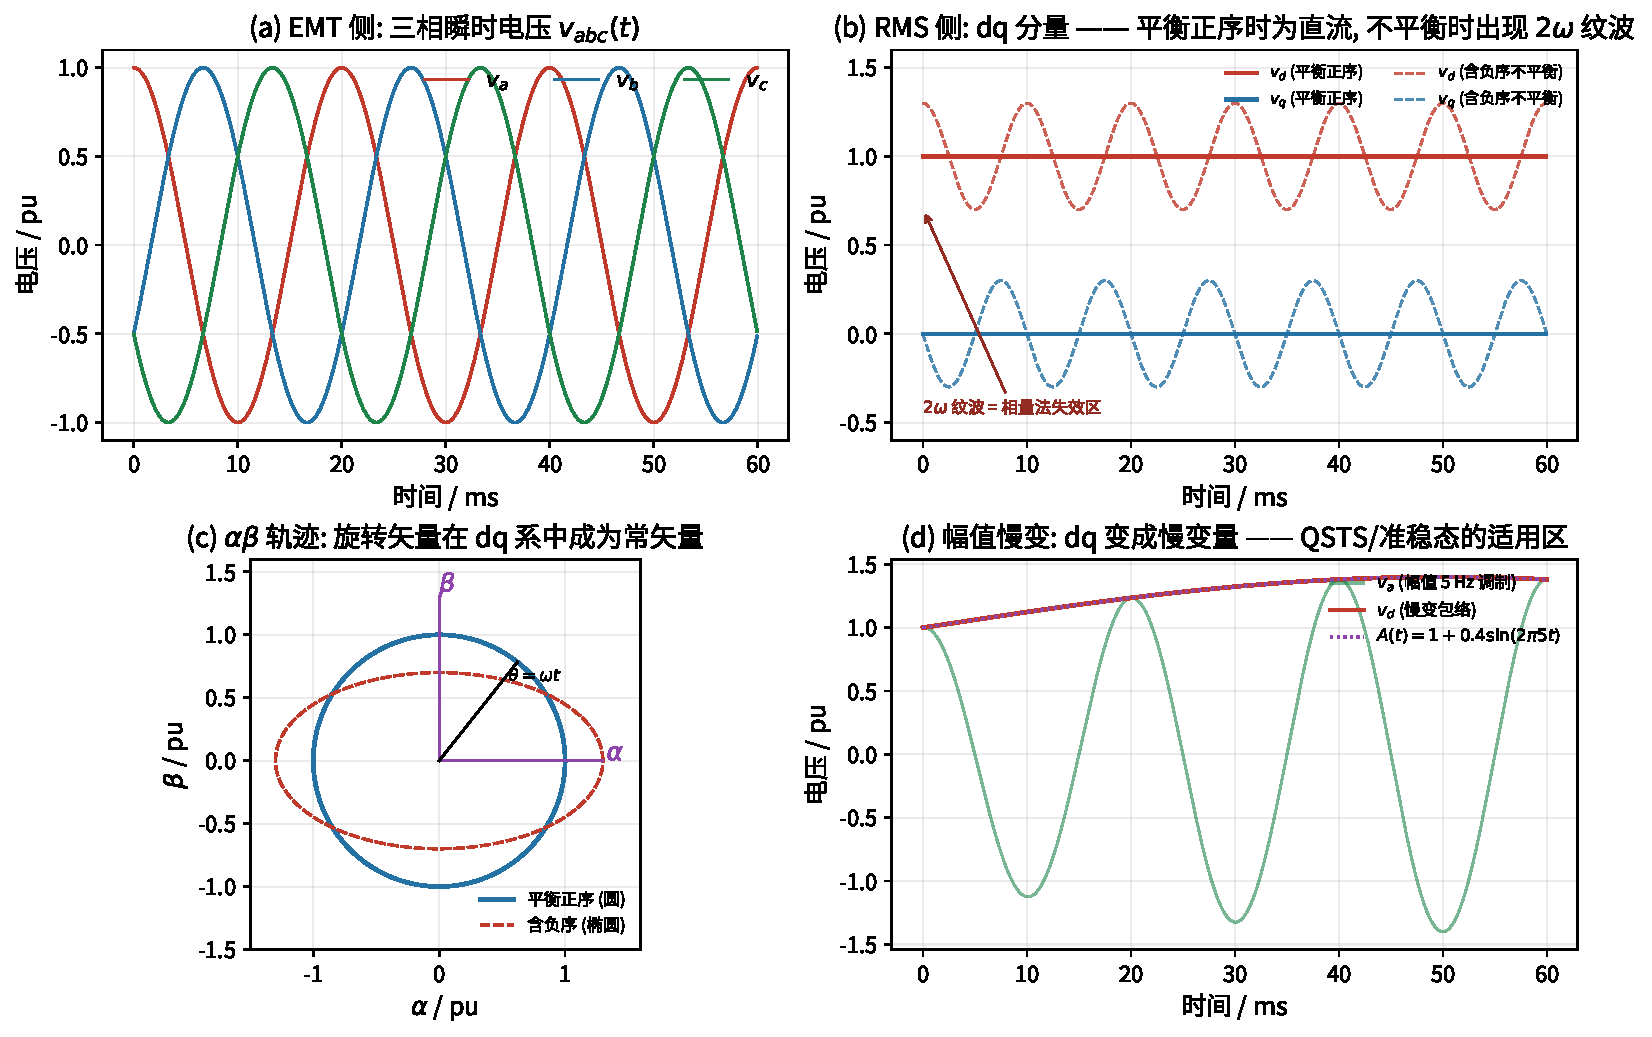
\includegraphics[width=0.98\textwidth]{fig03_park_transform.pdf}
\caption{\textbf{这张图说明}：为什么可以只盯住缓慢变化的幅值与相位，而把 50 Hz 的摆动“转掉”。
\textbf{画的是什么}：(a) 三相瞬时电压 $v_a,v_b,v_c$（三条正弦，横轴为时间 ms）；
(b) $dq$ 分量，实线为平衡正序、虚线为含负序的不平衡情形；
(c) $\alpha\beta$ 平面上的矢量轨迹（实线为圆、虚线为椭圆）；
(d) 幅值受 5 Hz 调制时的 $v_a$（细线）、其 $d$ 分量 $v_d$（粗线）与调制函数 $A(t)$（点线）。
\textbf{怎么读}：平衡正序时 $v_d$ 为水平直线、$v_q=0$（载波被“转掉”）；
含负序时 $dq$ 出现 $2\omega_s$ 纹波；幅值慢变时 $dq$ 变为慢变量。
\textbf{结论}：纹波说明三相不平衡时相量法失效；慢变说明准稳态/QSTS 的适用区。}
\label{fig:park}
\end{figure}


\subsubsection{RL 支路的 $dq$ 方程：交叉耦合项从哪来}
\begin{derivblock}{推导块 2：RL 支路的 dq 方程}
\textbf{起点}：$abc$ 域 $RL$ 方程；\textbf{目标}：$dq$ 形式与交叉项来源（2 步）；\textbf{结论}：$\omega L$ 来自坐标旋转、非电磁暂态；\textbf{支撑}：EMT/RMS 的分界。



由 $v_{abc}=Ri_{abc}+L\,\dd i_{abc}/\dd t$ 与 $\bm i_{abc}=\bT^{-1}\bm i_{dq0}$ 可得（完整推导见附录~\ref{app:rldq}）
\begin{equation}
\boxed{\;
v_d=R\,i_d+L\,\dif{i_d}{t}-\omega L\,i_q,\qquad
v_q=R\,i_q+L\,\dif{i_q}{t}+\omega L\,i_d .\;}
\label{eq:rl-dq}
\end{equation}
式~\eqref{eq:rl-dq} 是理解“EMT 与 RMS 差在哪”的钥匙：\\
RMS 保留 $\omega L$ 交叉项（它来自坐标旋转，不是电磁暂态），
但忽略 $L\,\dd i_d/\dd t$（它才是电磁暂态）；
EMT 两项都保留。若忽略哪一项，必须用 \S\ref{sec:quasi} 的判据量化。


\end{derivblock}

\subsubsection{准稳态（相量）近似与误差判据}
\begin{derivblock}{推导块 3：准稳态误差判据}
\textbf{起点}：复包络；\textbf{目标}：误差公式（3 步）；\textbf{结论}：$\varepsilon=m(\Omega/\omega_s)\sin\phi_z$；\textbf{支撑}：QSTS 是否可用的判据。

\textbf{与块 1 的衔接}：块 1（Park）说明了载波为什么可以“丢掉”；本块回答接下来的问题——
忽略包络的导数 $\dot I$ 会带来多大误差。其零阶结果就是工程上的相量法（动态相量法的零阶近似\cite{chen2023}）。


\label{sec:quasi}

设电源含慢变包络，$v(t)=\Real\{V(t)e^{\jj\omega_s t}\}$，把 $i(t)=\Real\{I(t)e^{\jj\omega_s t}\}$
代入 $v=Ri+L\,\dd i/\dd t$。由于 $\dd i/\dd t=\Real\{(\dot I+\jj\omega_s I)e^{\jj\omega_s t}\}$，
在基频分量上取等（即忽略 $I(t)$ 产生的 $2\omega_s$ 谐波）：
\begin{equation}
\underbrace{(R+\jj\omega_s L)}_{Z(\jj\omega_s)}I(t)\;+\;L\,\dot I(t)=V(t).
\label{eq:envelope-ode}
\end{equation}
\textbf{读法}：这是 $RL$ 支路在复包络下的\textbf{精确}方程；
与相量形式的差别只在多出的 $L\dot I$ 项——它正是相量法丢掉的那部分。
\textbf{相量法/准稳态法}就是令 $\dot I=0$：
\begin{equation}
I_0(t)=\frac{V(t)}{Z(\jj\omega_s)},\qquad
Z(\jj\omega_s)=R+\jj\omega_s L,\quad |Z|=\sqrt{R^2+(\omega_s L)^2}.
\label{eq:quasi-static}
\end{equation}
\textbf{读法}：令 $\dot I=0$ 得到熟悉的“复数欧姆定律”——这就是工程上的相量法；
$Z(\jmath\omega_s)$ 把电阻与电抗合并成一个复数。
对式~\eqref{eq:envelope-ode} 做一次收缩迭代：记 $I=I_0+\delta I$，零阶解为
式~\eqref{eq:quasi-static} 的 $I_0=V/Z$；代回并保留到一阶得 $Z\,\delta I\approx-L\dot I_0$，
即 $\delta I=-L\dot I_0/Z$。设 $V(t)=V_0(1+m\sin\Omega t)$，
则 $\dot I_0=m\Omega V_0\cos(\Omega t)/Z$，$|\dot I_0|_{\max}=m\Omega|I_0|$，于是相对误差
\begin{equation}
\boxed{\;
\varepsilon_{\text{qs}}
=\frac{|\delta I|_{\max}}{|I_0|}
=m\,\frac{\Omega}{\omega_s}\,\frac{\omega_s L}{|Z|}
=m\,\frac{\Omega}{\omega_s}\,\sin\phi_z ,
\qquad \phi_z=\arctan\frac{\omega_s L}{R} .\;}
\label{eq:qs-error}
\end{equation}
式~\eqref{eq:qs-error} 是本报告最重要的判据之一（同类误差机理在动态相量--电磁暂态混合仿真中的系统分析见文献\cite{chen2023}）：\textbf{准稳态误差正比于
“包络带宽 / 载波频率”，比例系数为 $\sin\phi_z\le1$}。
它同时解释了为什么
(i) 开关频率越高（$f_{\max}$ 越大）越不能用相量；
(ii) 当 $R\gg\omega_s L$（阻性主导）时 $\sin\phi_z\to0$，即便慢变也很准；
(iii) 当 $\omega_s L\gg R$（感性主导）时 $\sin\phi_z\to1$，误差最大，需 $\Omega/\omega_s\lesssim\varepsilon$。

\end{derivblock}

\begin{figure}[htbp]
\centering
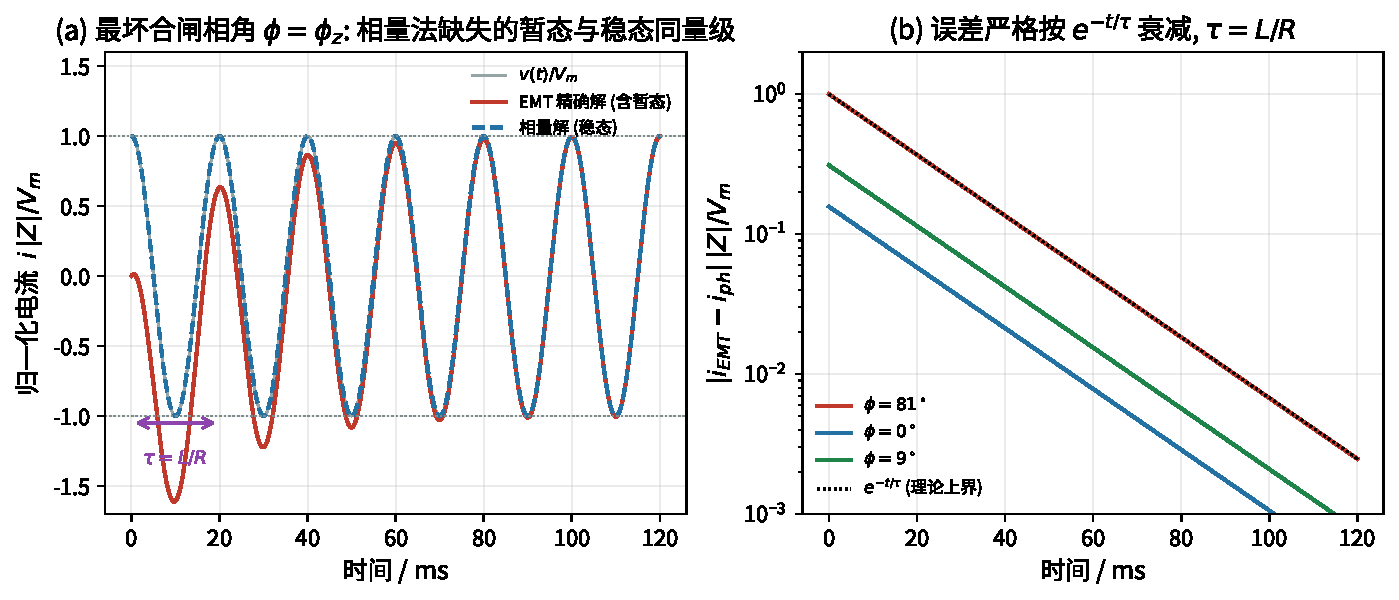
\includegraphics[width=0.98\textwidth]{fig04_phasor_vs_waveform.pdf}
\caption{\textbf{这张图说明}：相量法在最坏情况下会漏掉多大的量。
\textbf{画的是什么}：(a) 横轴为时间（ms），纵轴为归一化电流 $i|Z|/V_m$，
其中 $|Z|=\sqrt{R^2+(\omega_sL)^2}$ 为阻抗模、$V_m$ 为电压峰值；
灰细线为电源电压、红线为 EMT 精确解（含暂态）、蓝虚线为相量稳态解。
(b) 纵轴为两解之差（对数），三条曲线对应不同合闸相角 $\phi$（电压初相），黑点线为理论衰减 $e^{-t/\tau}$。
参数：$\omega_s=2\pi\times50$ rad/s，$R=1\,\Omega$，$L=0.02$ H，故 $\tau=L/R=20$ ms、$\omega_sL/R\approx6.3$。
\textbf{怎么读}：(a) 两解在稳态段重合、在起始段分离，分离量就是被丢掉的直流暂态；(b) 差值按 $e^{-t/\tau}$ 衰减。
\textbf{结论}：最坏合闸角（$\phi=\phi_z$，$\phi_z=\arctan(\omega_sL/R)$）下，丢掉的暂态与稳态分量同量级。}
\label{fig:phasor}
\end{figure}

解析地，$L\,\dd i/\dd t+R i=V_m\cos(\omega_s t+\phi)$、$i(0)=0$ 的解为
\begin{equation}
i_{\text{EMT}}(t)=\frac{V_m}{|Z|}\Bigl[\cos(\omega_s t+\phi-\phi_z)
-\cos(\phi-\phi_z)e^{-t/\tau}\Bigr],\quad \tau=\frac{L}{R},
\label{eq:phasor-exact}
\end{equation}
\textbf{读法}：方括号内第一项是稳态（相量）解，第二项是合闸产生的直流暂态，
按 $e^{-t/\tau}$ 衰减；相量法只保留了第一项。
而相量解是其中的稳态项。两者之差为
$\frac{V_m}{|Z|}\cos(\phi-\phi_z)e^{-t/\tau}$，
在 $\phi=\phi_z$（最坏合闸角）时幅值等于稳态幅值——这就是图~\ref{fig:phasor}(a) 的现象。

\begin{figure}[htbp]
\centering
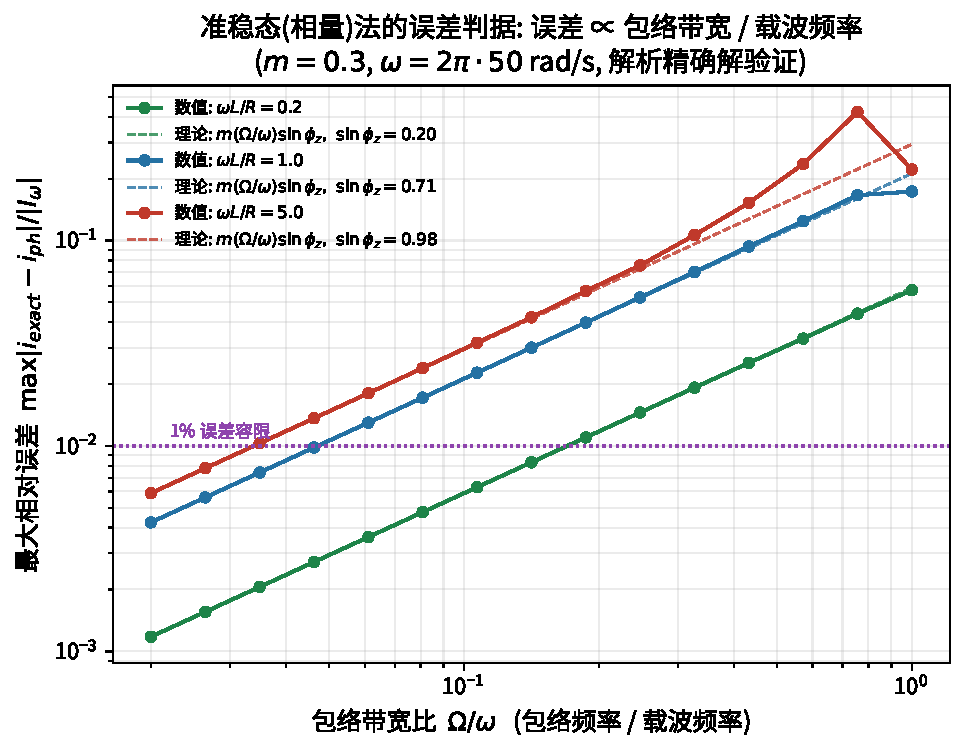
\includegraphics[width=0.99\textwidth]{fig05_quasistatic_error.pdf}
\caption{\textbf{这张图说明}：什么时候可以放心用相量法（潮流/QSTS），什么时候不行。
\textbf{画的是什么}：横轴为带宽比 $\Omega/\omega_s$（对数；$\Omega$ 为电压包络的变化角频率，$\omega_s=2\pi\times50$ rad/s）；
纵轴为最大相对误差 $\max|i_{\text{精确}}-i_{\text{相量}}|/|I_0|$（对数）。
三组曲线对应不同的 $\omega_sL/R$（感抗与电阻之比，取 $0.2,\,1,\,5$）；
每组中带点线为数值结果、细虚线为解析式 $\varepsilon=m(\Omega/\omega_s)\sin\phi_z$
（$m=0.3$ 为包络调制深度，$\phi_z=\arctan(\omega_sL/R)$）；水平点线为 $1\%$ 误差容限。
\textbf{怎么读}：三组曲线斜率均为 1，说明误差与带宽比成正比；数值与理论重合即验证了公式。
\textbf{结论}：准稳态误差判据式~\eqref{eq:qs-error} 成立，可由它与误差容限反推允许的带宽比。}
\label{fig:quasistatic}
\end{figure}

\paragraph{小问题：准稳态误差式~\eqref{eq:qs-error} 是怎么来的、量级多大？}
它来自“复包络 $+$ 一次收缩迭代”：把 $v=\Real\{Ve^{\jmath\omega_s t}\}$、
$i=\Real\{Ie^{\jmath\omega_s t}\}$ 代入 $v=Ri+L\dot i$，
先算忽略 $\dot I$ 的零阶解 $I_0=V/Z$，再把 $I_0$ 代回右端得到一阶修正
$\delta I=-L\dot I_0/Z$，于是相对误差为
$|\delta I|/|I_0|=m(\Omega/\omega_s)\cdot(\omega_sL/|Z|)$。
量级上，$m\sim0.3$、$\Omega/\omega_s\sim0.1$ 时误差约 $3\%$，
与图~\ref{fig:quasistatic} 的数值一致；
要让误差低于 $1\%$，需 $\Omega/\omega_s<0.01/(m\sin\phi_z)$。


\subsection{第三层：为什么可以这样连接（奇异摄动与慢流形）}
\begin{derivblock}{推导块 4：奇异摄动与慢流形}
\textbf{起点}：$\varepsilon\dot{\bm z}=\bm g(\bm x,\bm z)$；\textbf{目标}：慢流形与降阶（3 步）；\textbf{结论}：RMS $=$ EMT 在 $\varepsilon\to0$ 的降阶；\textbf{支撑}：前两层连接的合法性。

\textbf{与块 2、块 3 的关系}：块 2、块 3 处理的是“某一条支路”上的快慢分离；
本块把它推广到一般系统，因此\textbf{块 3 的准稳态近似就是本框架的零阶结果}——
两者是同一件事的“具体实例”与“统一表述”，不是两套独立结论。


\label{sec:singular}

把完整系统按时间尺度分成慢变量 $\bx$（机电，秒级）与快变量 $\bz$（电磁，$\mu$s--ms 级），
写成标准奇异摄动形式
\begin{equation}
\dot\bx=\bm{f}(\bx,\bz),\qquad
\varepsilon\,\dot\bz=\bm{g}(\bx,\bz),\qquad
0<\varepsilon\ll1 .
\label{eq:singular}
\end{equation}
\textbf{读法}：$\varepsilon$ 是快慢时间常数之比；第二式左端被 $\varepsilon$ 压小，
意味着 $\bz$ 相对 $\bx$ 几乎是“瞬间”跟随。
令 $\varepsilon\to0$ 得\textbf{代数约束} $\bm{g}(\bx,\bz)=\bzero$；
若 $\partial\bm{g}/\partial\bz$ 可逆（等价于快子系统稳定），由隐函数定理得\textbf{慢流形}
\begin{equation}
\bz=\bm{h}(\bx),\qquad
\dot\bx=\bm{f}\bigl(\bx,\bm{h}(\bx)\bigr)=:\bm{f}_r(\bx).
\label{eq:slow-manifold}
\end{equation}
\textbf{读法}：快变量不再独立演化，而是被慢变量\textbf{完全决定}——
这就是“降阶”：去掉了快变量对应的微分方程，换成代数约束。
式~\eqref{eq:slow-manifold} 就是\textbf{降阶模型}。Tikhonov 定理给出误差界：
若快子系统在流形邻域内一致渐近稳定，则原解在 $O(\varepsilon)$ 时间（边界层）内经
$\|\bz(t)-\bm{h}(\bx(t))\|\le C e^{-t/\varepsilon}$ 收敛到降阶解，之后误差为 $O(\varepsilon)$。

\end{derivblock}

\begin{figure}[htbp]
\centering
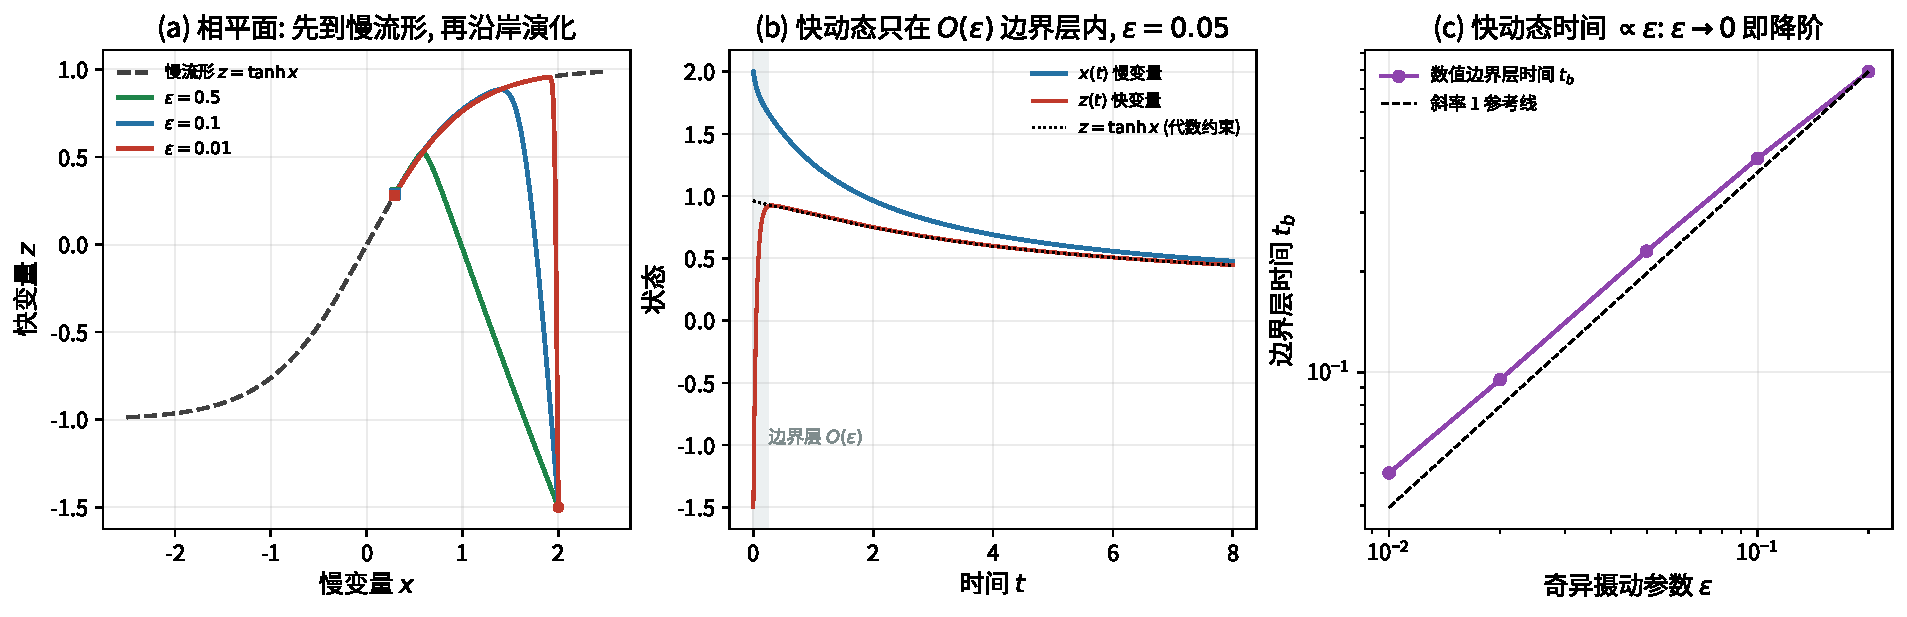
\includegraphics[width=0.99\textwidth]{fig06_singular_perturbation.pdf}
\caption{\textbf{这张图说明}：为什么可以把“变化太快”的东西忽略掉而不出错。
\textbf{画的是什么}：(a) 相平面 $(x,z)$，$x$ 为慢变量、$z$ 为快变量；黑虚线为慢流形 $z=\tanh x$，
三条彩色曲线为 $\varepsilon=0.5,\,0.1,\,0.01$ 的轨迹（圆点为起点、方点为终点）。
(b) 一条轨迹（$\varepsilon=0.05$）的 $x(t)$、$z(t)$ 与代数约束 $\tanh x$，阴影为边界层。
(c) 边界层时间 $t_b$（$z$ 进入慢流形邻域所需时间）与 $\varepsilon$ 的双对数关系及斜率 1 参考线。
所演示的系统为 $\dot x=-x+z$、$\varepsilon\dot z=\tanh x-z$。
\textbf{怎么读}：$\varepsilon$ 越小，轨迹越快贴到慢流形（先竖直、再沿流形）；$t_b$ 与 $\varepsilon$ 成正比。
\textbf{直观理解}：把快变量 $z$ 想成一个很灵敏的温度计、慢变量 $x$ 是室温，$\varepsilon$ 相当于温度计的响应时间。
$\varepsilon$ 很小 → 温度计几乎瞬间读数（轨迹立刻贴到慢流形、边界层很薄）；
$\varepsilon$ 变大 → 温度计要过一会儿才追上（轨迹变成斜线）。
所以 $\varepsilon$ 决定“快动态能被忽略到什么程度”。
\textbf{结论}：$\varepsilon\to0$ 时快动态被代数约束替代——这是 RMS 由 EMT 降阶的数学结构。}
\label{fig:singular}
\end{figure}

\begin{figure}[htbp]
\centering
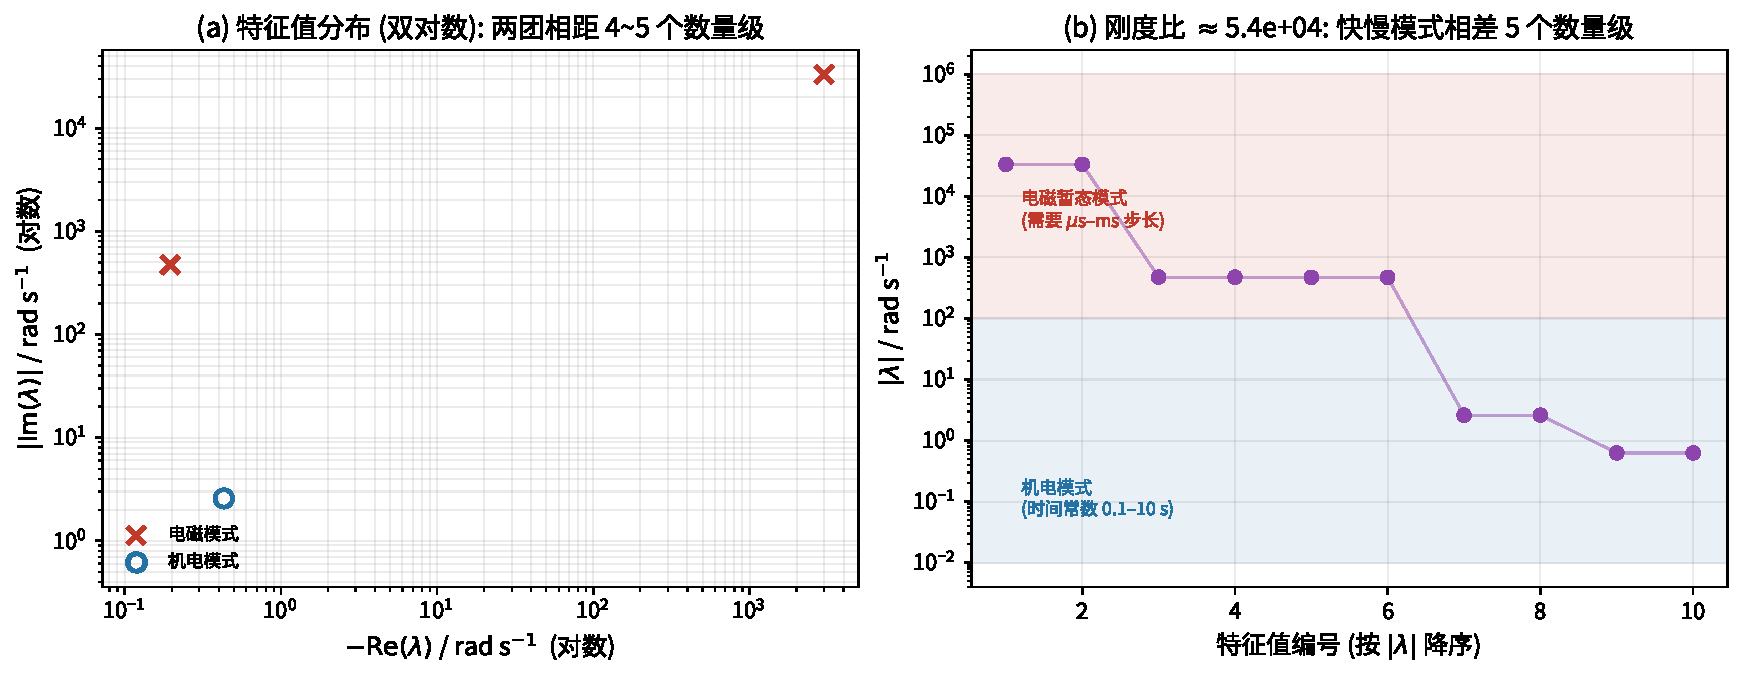
\includegraphics[width=0.98\textwidth]{fig07_eigen_spectrum.pdf}
\caption{\textbf{这张图说明}：为什么 EMT 这么慢、这么贵。
\textbf{画的是什么}：(a) 特征值 $\lambda$ 的分布，横轴为 $-\mathrm{Re}\,\lambda$、纵轴为 $|\mathrm{Im}\,\lambda|$（均为对数轴）；
红叉为电磁模式（$|\lambda|\sim10^4$ rad/s）、蓝圈为机电模式（$|\lambda|\sim10^0$ rad/s）。
(b) 按 $|\lambda|$ 降序排列的特征值（纵轴对数），红带为电磁区间、蓝带为机电区间。
算例为 $10$ 阶 $dq$ 模型：无穷大母线 $+$ 两段 RL 线路 $+$ 节点电容 $+$ 一台同步机（参数见脚本）。
\textbf{怎么读}：特征值分成两团、相隔 4--5 个数量级；两团之比即刚度比 $\kappa=\max|\lambda|/\min|\lambda|\approx5\times10^4$。
\textbf{直观理解}：最快的模态决定“步长至少要多小”，最慢的模态决定“总共要算多长”；
两者之比就是需要的步数——刚度比越大，步数越多、代价越高。
\textbf{结论}：刚度比决定全阶 EMT 必须同时用微秒级步长与秒级仿真窗口，计算量比 RMS 高 $10^{3}$--$10^{6}$ 倍。}
\label{fig:spectrum}
\end{figure}

\label{sec:eigen}
图~\ref{fig:spectrum} 的算例把 $\varepsilon$ 具体化为刚度比
\begin{equation}
\varepsilon_{\text{grid}}\;\sim\;\frac{\tau_{\text{em}}}{\tau_{\text{mech}}}
=\frac{L/R}{M/D}\;\sim\;10^{-4}\text{--}10^{-6},
\label{eq:eps-grid}
\end{equation}
\textbf{读法}：电网的 $\varepsilon$ 就是“电磁时间常数 $\div$ 机电时间常数”，量级 $10^{-4}$--$10^{-6}$；
$\varepsilon$ 越小，降阶越安全，但 EMT 要付出的计算代价越大。

（与 \S\ref{sec:q1} 中“EMT 计算量高 $10^{3}$--$10^{6}$ 倍”的估计一致。）

\paragraph{小问题：刚度比 $5\times10^4$ 是怎么算出来的？真实电网是多少？}
它不是估的，是对一个 $10$ 阶 $dq$ 模型（无穷大母线 $+$ 两段 RL 线路 $+$ 节点电容
$+$ 一台同步机）先数值求平衡点、再数值求 Jacobian 特征值得到的，
脚本为 \texttt{fig07\_spectrum.py}，全部参数写在文件中。
真实系统若含变流器开关级模式，快速模式可达 $10^6$ rad/s 以上，
因此报告统一写“$10^4$--$10^6$”。这个区间正是“EMT 计算量高
$10^3$--$10^6$ 倍”的来源。


\subsection{工程推广：混合仿真的接口与代价}
\label{sec:hybrid}

当需要一个区域用 EMT、其余用 RMS 时，就出现\textbf{接口}问题
（相关实现与研究见文献\cite{huang2017,liu2024}）。
图~\ref{fig:hybrid} 给出结构与时步关系。接口交换的变量是明确的：
\begin{equation}
\underbrace{\bigl\{v_{abc}(t),\,i_{abc}(t)\bigr\}}_{\text{EMT 侧瞬时量}}
\;\xrightarrow[\text{滑动 DFT}]{\ \ \text{基频提取}\ \ }\;
\underbrace{\bigl\{V\angle\theta,\ I\angle\theta\bigr\}}_{\text{RMS 侧相量}}
\;\xrightarrow[\text{相量合成}]{\ \ \text{受控源}\ \ }\;
\underbrace{\bigl\{v_{abc}(t)\bigr\}}_{\text{EMT 侧瞬时量}} .
\label{eq:interface-vars}
\end{equation}
\textbf{读法}：接口两边交换的量是明确的——EMT 侧给出瞬时波形、接收相量；
RMS 侧给出相量、接收瞬时波形；中间的滑动 DFT 与相量合成就是双向翻译器。
接口处的功率必须守恒：三相瞬时功率在一个周期上的平均应等于相量功率
\begin{equation}
P=\frac{1}{T}\int_{t-T}^{t}\sum_{\varphi\in\{a,b,c\}}\!\!v_\varphi(\tau)i_\varphi(\tau)\,\dd\tau
\;\overset{\text{平衡正序}}{=}\;\frac{3}{2}\bigl(v_d i_d+v_q i_q\bigr)
\;\overset{\text{相量}}{=}\;\Real\{V I^{*}\}\times3 .
\label{eq:power-consistency}
\end{equation}
\textbf{读法}：三种写法必须相等——第一个等号是“一个周期的瞬时平均”，
第二个等号用幅值不变的 $dq$ 变换（$v_d,i_d$ 为峰值），第三个等号假定 $V,I$ 为\textbf{有效值相量}。
它是接口“不产生虚假功率”的校验式，实现后应逐时步检查。
接口等值电路通常取\textbf{诺顿/戴维南等值}：EMT 侧把 RMS 区域看作
“电流源 $I_n$ 并联导纳 $Y_n$”，RMS 侧把 EMT 区域看作“电压源 $E_{th}$ 串联阻抗 $Z_{th}$”。
这两组等值参数不是任意的，它们决定了接口的数值稳定性（本质是阻抗匹配问题）。

\begin{figure}[htbp]
\centering
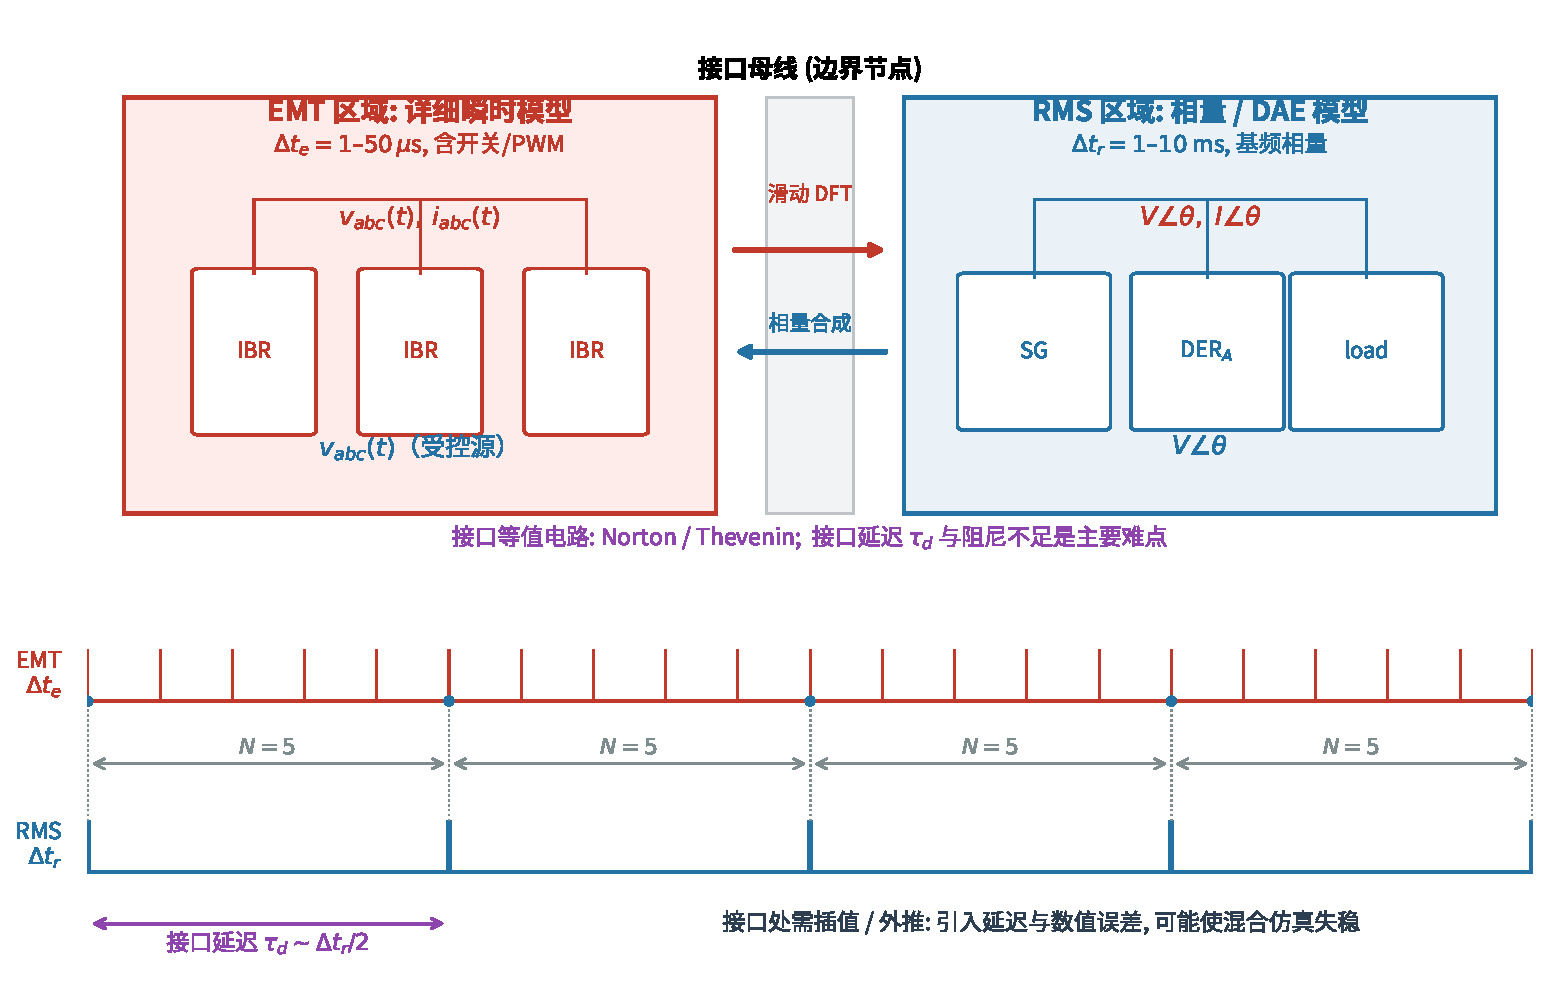
\includegraphics[width=0.98\textwidth]{fig08_hybrid_interface.pdf}
\caption{\textbf{这张图说明}：EMT 和 RMS 拼在一起时，两边到底交换什么、代价是什么。
\textbf{看图}：红区为 EMT 侧、蓝区为 RMS 侧，中间灰带为接口母线；
红箭头是 EMT$\to$RMS（滑动 DFT 提取相量），蓝箭头是 RMS$\to$EMT（相量合成受控源）；
下图为双时间轴，一个 RMS 大步含 $N$ 个 EMT 小步，紫色箭头标出接口延迟 $\tau_d\sim\Delta t_r/2$。
\textbf{直观理解}：RMS 侧在一个大步内把接口值“记住不动”，而 EMT 侧一直在变；
直到下一个交换时刻才更新，等效于平均慢半个大步——这就是延迟的来源。
\textbf{结论}：接口交换的量就是图上标注的 $v_{abc},i_{abc}$ 与 $V\angle\theta,I\angle\theta$；
代价是延迟与插值误差。}
\label{fig:hybrid}
\end{figure}

\begin{figure}[htbp]
\centering
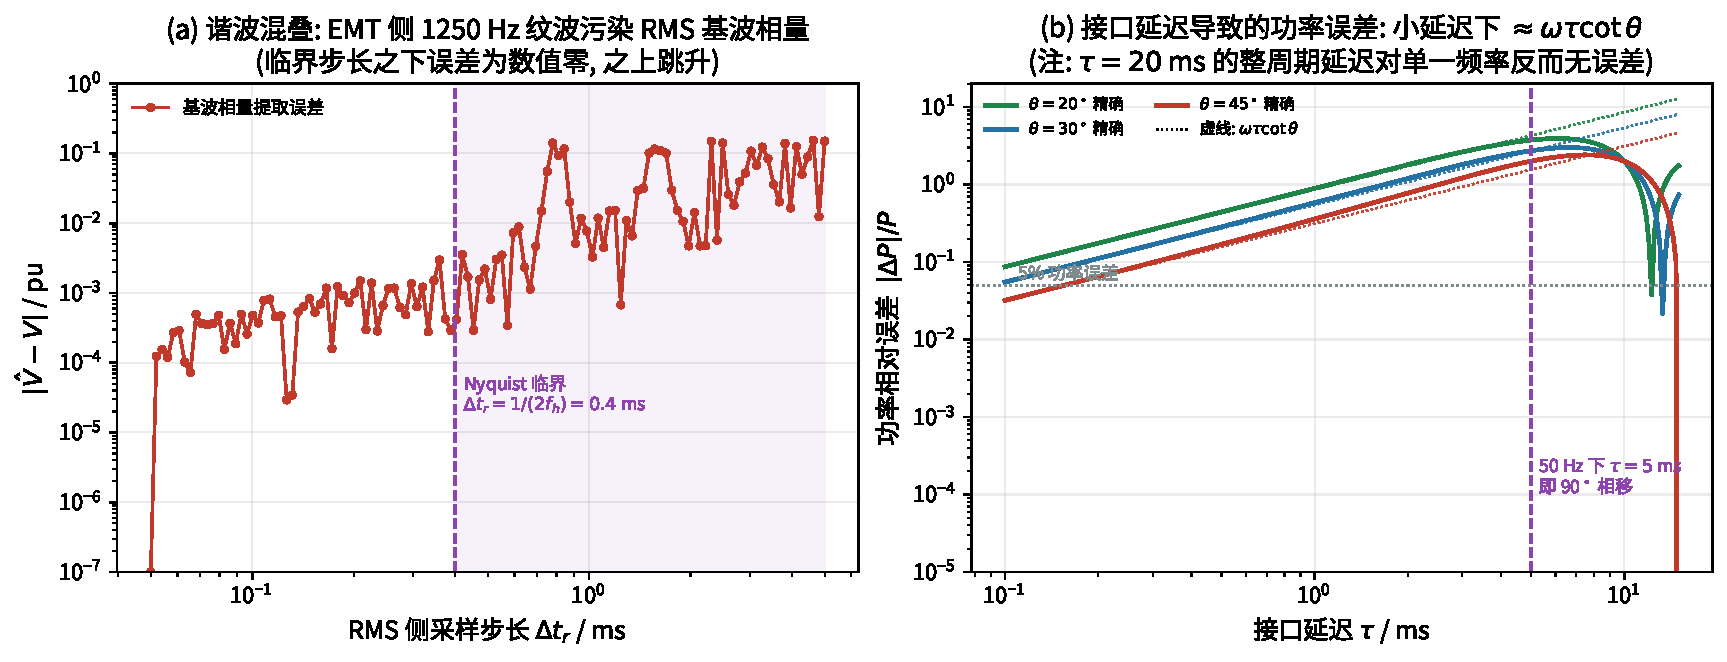
\includegraphics[width=0.98\textwidth]{fig09_interface_error.pdf}
\caption{\textbf{这张图说明}：拼接口时，哪些坑会让结果不可信。
\textbf{画的是什么}：(a) 横轴为 RMS 侧采样步长 $\Delta t_r$（对数，ms），
纵轴为基波相量提取误差 $|\hat V-V|$（对数）；红点线为数值结果，
紫色竖线为 Nyquist 临界 $\Delta t_r=1/(2f_h)=0.4$ ms（$f_h$ 为 EMT 侧最高关心谐波，这里取 $1250$ Hz），阴影为混叠区。
(b) 横轴为接口延迟 $\tau$（对数，ms），纵轴为功率相对误差 $|\Delta P|/P$（对数）；
三条实线为不同相角差 $\theta$ 下的精确值（功率 $P=(V_1V_2/X)\sin\theta$），
细点线为近似式 $\omega_s\tau\cot\theta$，竖线标注 $\tau=5$ ms，水平点线为 $5\%$ 误差。
\textbf{怎么读}：(a) 临界步长之下误差为数值零，超过后跳升；(b) 小延迟时精确值与近似式重合，
$\theta$ 越小（轻载）误差越大。
\textbf{直观理解}：(a) 采样太慢就像“看漏”了快速抖动，抖动会伪装成慢变化（混叠）；
(b) 延迟让相角“看晚了一步”，而功率对相角很敏感——所以延迟会造成明显功率误差，轻载时更明显。
\textbf{结论}：接口的两条硬约束——采样定理与延迟误差——决定混合仿真能否使用。}
\label{fig:interface}
\end{figure}

\paragraph{延迟误差的推导。} 若 RMS 侧输出给 EMT 的电压相量比真实值滞后时间 $\tau$，
则其相角估计滞后 $\Delta\theta=\omega_s\tau$。对两母线间功率
$P=(V_1V_2/X)\sin\theta$ 做一阶展开：
\begin{equation}
\frac{\Delta P}{P}
=\frac{\sin(\theta-\omega_s\tau)-\sin\theta}{\sin\theta}
\approx-\frac{\omega_s\tau\cos\theta}{\sin\theta}
=-\omega_s\tau\cot\theta ,
\label{eq:delay-error}
\end{equation}
其绝对值即图~\ref{fig:interface}(b) 中虚线。式~\eqref{eq:delay-error} 说明：
\textbf{接口延迟必须补偿，否则重载线路（$\theta$ 大、$\cot\theta$ 小）反而误差小，
而轻载/长线（$\theta$ 小）误差巨大}；这是一个反直觉但可直接验证的结论。
$50$ Hz 下 $\tau=5$ ms 对应 $\omega_s\tau=\pi/2$，即 $90^\circ$ 相移，足以使接口失稳。

\paragraph{小问题：接口传什么变量？步长比 $N$ 取多大？为什么轻载时延迟误差反而大？}
（i）\textbf{传什么}：EMT$\to$RMS 传三相瞬时 $v_{abc},i_{abc}$ 提取出的
基频相量 $V\angle\theta,I\angle\theta$；RMS$\to$EMT 传相量合成的受控源 $v_{abc}(t)$
（式~\eqref{eq:interface-vars}），接口功率按一个周期平均守恒（式~\eqref{eq:power-consistency}）。
（ii）\textbf{$N$ 取多大}：$N=\Delta t_r/\Delta t_e$ 的上限由接口精度与稳定性决定，不是越大越好。
例：若 EMT 侧最高关心谐波为 $1250$ Hz，则 $\Delta t_r<0.4$ ms（式~\eqref{eq:nyquist}），
取 $\Delta t_e=50\,\mu$s 时 $N\le8$；若 EMT 侧含 $10$ kHz 开关级细节，则 $\Delta t_r<0.05$ ms，
必须减小 $N$，或先在 EMT 侧滤波再送入接口。
（iii）\textbf{为什么轻载更敏感}：延迟是相角误差，而 $P=(V_1V_2/X)\sin\theta$
对相角的灵敏度是 $\cos\theta$；$\theta$ 小时 $\cot\theta$ 很大，
相对误差 $\omega_s\tau\cot\theta$ 被放大（图~\ref{fig:interface}b）。

\paragraph{采样定理。} 设 EMT 侧最高关心谐波为 $f_h$，则 RMS 侧采样步长必须满足
\begin{equation}
\Delta t_r<\frac{1}{2f_h}
\qquad\bigl(f_h=1250\,\text{Hz}\Rightarrow \Delta t_r<0.4\,\text{ms}\bigr),
\label{eq:nyquist}
\end{equation}
否则该谐波会混叠到基波频带，污染相量（图~\ref{fig:interface}a）。
这与“RMS 步长可以取 $10$ ms”的直觉矛盾：步长上限不是由机电动态决定，而是由
\textbf{接口精度}决定——这也是混合仿真中“RMS 侧也必须用较小步长”的原因。

\section{Q4：Kuramoto 模型与电网——为什么能用、代价是什么（重点）}
\label{sec:q4}

\noindent\textbf{本章回答}：Kuramoto 为什么能用于电网、假设是什么、与 RMS 是什么关系。
逻辑是“先建模型、再证明它从哪来、最后划清边界”：先给标准形式与变量含义，
再从 swing 方程逐步推出它，最后给出可解析结论与适用边界。

\subsection{模型形式与变量含义}

Kuramoto 模型描述 $N$ 个弱耦合、近全同的相位振子\cite{kuramoto1984}：
\begin{equation}
\dot\theta_i=\omega_i+\frac{K}{N}\sum_{j=1}^{N}\sin(\theta_j-\theta_i),
\qquad i=1,\dots,N,
\label{eq:kuramoto}
\end{equation}
\textbf{读法}：每个振子按自身的自然频率 $\omega_i$ 转动，同时被耦合项“拉”向与其他振子一致的相位；
$K$ 越大，拉得越紧。
其中三个量的物理含义是
\begin{center}
\begin{tabular}{@{}ll@{}}
\toprule
符号 & 含义 \\
\midrule
$\theta_i$ & 第 $i$ 个振子的相位（在电网中对应节点电压相角或机组转子角） \\
$\omega_i$ & 自然频率（无耦合时该振子自由振荡的频率；电网中对应节点有功不平衡） \\
$K$ & 耦合强度（电网中对应线路电纳/电抗，$K_{ij}=V_iV_jB_{ij}$） \\
\bottomrule
\end{tabular}
\end{center}
描述宏观同步程度用\textbf{序参量}
\begin{equation}
r e^{\jj\psi}=\frac{1}{N}\sum_{j=1}^{N}e^{\jj\theta_j},\qquad r\in[0,1],
\label{eq:order-param}
\end{equation}
\textbf{读法}：$r=0$ 表示完全无序，$r=1$ 表示完全同步，$\psi$ 为平均相位——
用一个标量概括整个网络的同步程度。
由于式~\eqref{eq:kuramoto} 的耦合项可写成
$\frac{K}{N}\sum_j\sin(\theta_j-\theta_i)
=K\,\Imag\bigl[e^{-\jj\theta_i}\frac{1}{N}\sum_j e^{\jj\theta_j}\bigr]
=K r\sin(\psi-\theta_i)$，
全连接 Kuramoto 可用\textbf{平均场}精确积分（每步只需 $O(N)$）：
\begin{equation}
\dot\theta_i=\omega_i+K\,r(t)\sin\bigl(\psi(t)-\theta_i\bigr).
\label{eq:kuramoto-meanfield}
\end{equation}
\textbf{读法}：耦合被压缩成“与平均场的相互作用”，每步只需 $O(N)$——
这正是 Kuramoto 可解析、可做大规模数值实验的原因。
这正是本报告 \texttt{fig11} 数值实验的计算方式。

\subsection{为什么能用于电网：从 swing 方程到 Kuramoto（假设 A1--A3）}
\begin{derivblock}{推导块 5：从 swing 方程到 Kuramoto}
\textbf{起点}：swing 方程 $+$ 网络功率；\textbf{目标}：三假设下的退化（3 步）；\textbf{结论}：Kuramoto 是 swing 的严格退化；\textbf{支撑}：Q4“为什么能用”。



\paragraph{第一步：转子运动方程。}
同步机的二阶经典模型为\cite{anderson2003,kundur1994}
\begin{equation}
\dot\delta_i=\omega_i-\omega_s,\qquad
M_i\,\dot\omega_i=P_{m,i}-P_{e,i}-D_i(\omega_i-\omega_s),
\label{eq:swing}
\end{equation}
$M_i$ 为惯性常数，$D_i$ 为阻尼，$P_{m,i}$ 为机械功率，$P_{e,i}$ 为电磁功率。
\textbf{读法}：第一式给出相角与转速的关系；第二式是转子运动方程——
不平衡功率（$P_m-P_e$）驱动转速变化，阻尼 $D$ 抑制振荡。

\paragraph{第二步：电磁功率的网络表达。} 由式~\eqref{eq:power-flow}，
节点 $i$ 的有功注入为
\begin{equation}
P_{e,i}=V_i^2G_{ii}+\sum_{j\neq i}V_iV_j\bigl(G_{ij}\cos\delta_{ij}+B_{ij}\sin\delta_{ij}\bigr),
\qquad \delta_{ij}=\delta_i-\delta_j .
\label{eq:Pe-general}
\end{equation}
\textbf{读法}：电磁功率由网络导纳与所有相角差共同决定——
网络约束就是在这里进入动力学方程的。

\paragraph{第三步：三个假设。} 在\textbf{（A1）无损}（$G_{ij}=0$）、
\textbf{（A2）电压幅值恒定}（$V_i\equiv V$）、
\textbf{（A3）均匀惯性/阻尼}（$M_i\equiv M$，$D_i\equiv D$）的条件下
（这一化简在文献\cite{filatrella2008,dorfler2012}中被严格讨论），
式~\eqref{eq:Pe-general} 退化为
\begin{equation}
P_{e,i}=\sum_{j\neq i}K_{ij}\sin\delta_{ij},\qquad K_{ij}=V_iV_jB_{ij}=\frac{V_iV_j}{X_{ij}} .
\label{eq:Pe-lossless}
\end{equation}
\textbf{读法}：在 A1、A2 下只剩 $\sin$ 项；耦合强度 $K_{ij}=V_iV_j/X_{ij}$
完全由电压幅值与线路电抗决定，与运行点无关。
把式~\eqref{eq:Pe-lossless} 代入式~\eqref{eq:swing}：
\begin{equation}
\boxed{\;
M_i\ddot\delta_i=P_{m,i}-\sum_{j\neq i}K_{ij}\sin(\delta_i-\delta_j)-D_i\dot\delta_i\;}
\label{eq:swing-kuramoto}
\end{equation}
式~\eqref{eq:swing-kuramoto} 保留惯性，称为\textbf{二阶 Kuramoto}（含惯性的 swing 型）。
若进一步取\textbf{过阻尼极限} $M_i\to0$，则惯性项消失，化为一阶标准 Kuramoto 式~\eqref{eq:kuramoto}。
因此：
\begin{quote}
\textbf{Kuramoto 模型不是“类比”，而是同步机摇摆方程在（A1）无损、（A2）恒幅值、
（A3）均匀惯性/过阻尼三个假设下的严格退化形式。}
其变量对应为：$\theta_i\leftrightarrow\delta_i$，
$\omega_i\leftrightarrow P_{m,i}/M_i$（或 $P_{m,i}/D_i$），
$K_{ij}\leftrightarrow V_iV_j/X_{ij}$。
\end{quote}

\end{derivblock}

\begin{figure}[htbp]
\centering
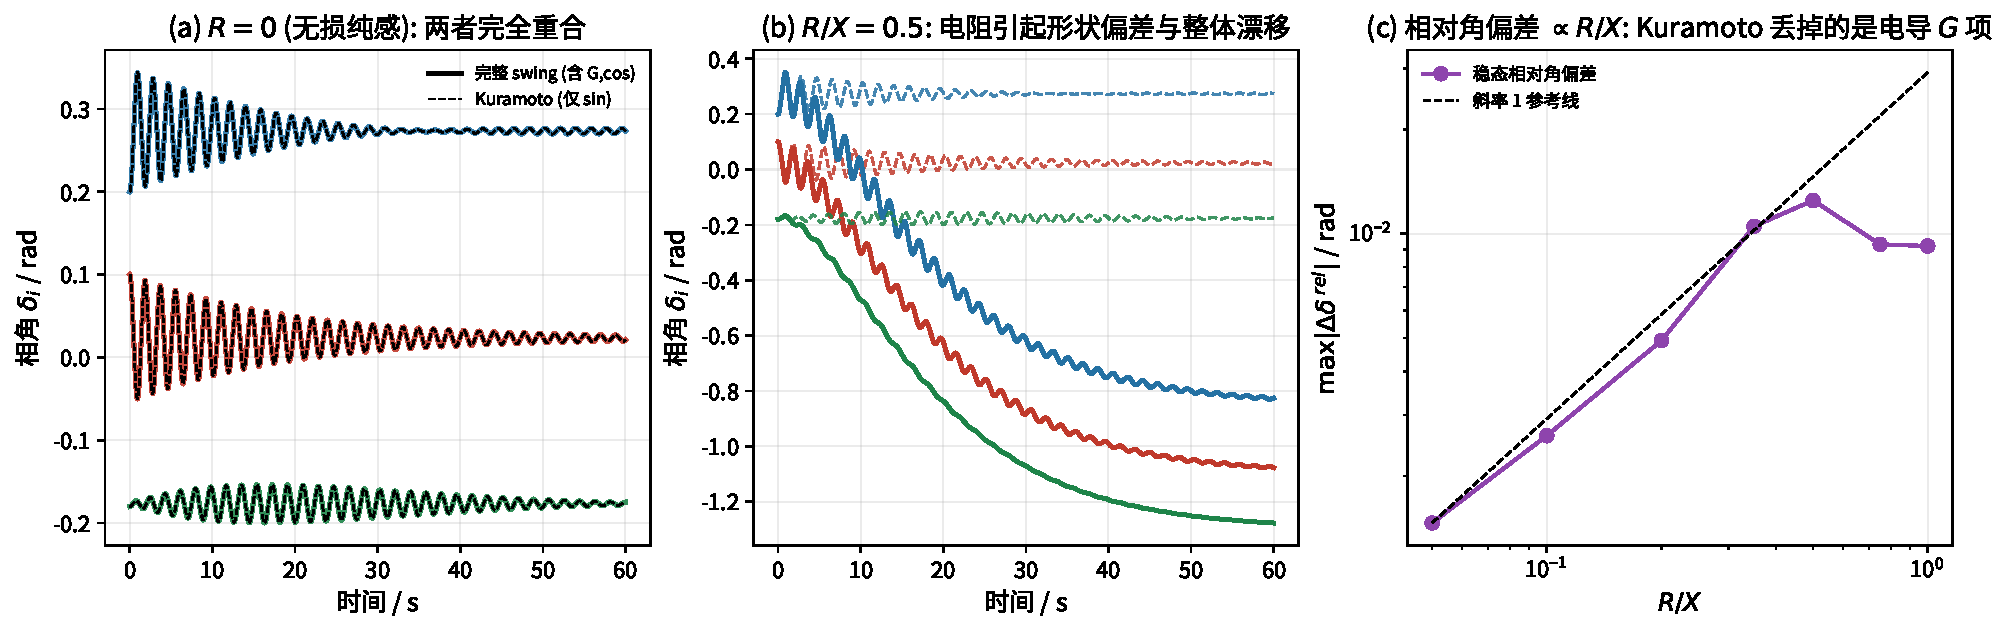
\includegraphics[width=0.99\textwidth]{fig10_swing_vs_kuramoto.pdf}
\caption{\textbf{这张图说明}：Kuramoto 与真实的电网模型差多少、在什么条件下完全一样。
\textbf{画的是什么}：(a) $R=0$ 时三台机组的转子角 $\delta_i(t)$（彩色实线为完整 swing 模型，黑色虚线为 Kuramoto 模型，两者重合）；
(b) $R/X=0.5$ 时两者分离（实线为完整模型、虚线为 Kuramoto）；
(c) 稳态相对角偏差（各时刻先减去整体均值再取最大）与 $R/X$ 的双对数关系及斜率 1 参考线。
$R,X$ 为线路电阻与电抗；假设 A1（无损）、A2（恒幅值）见 \S\ref{sec:q4}。
\textbf{怎么读}：(a) 两解完全重合，说明在假设 A1--A2 下 Kuramoto 是严格退化；
(b)(c) 电阻使两解分离，且相对角偏差与 $R/X$ 成正比。
\textbf{直观理解}：Kuramoto 只保留了“纯电抗”的耦合，电阻带来的那一部分被丢掉；
电阻相对电抗越大（$R/X$ 越大），丢掉的越多。
\textbf{结论}：Kuramoto 丢掉的是电导 $G$ 项；输电线路 $R/X\sim0.05$--$0.2$ 可接受，配电网 $R/X\sim1$--$5$ 不适用。}
\label{fig:swing}
\end{figure}

图~\ref{fig:swing} 的数值实验还揭示一个细节：
$R\neq0$ 时系统的整体相角会出现\textbf{中性漂移}（所有 $\delta_i$ 同时平移），
因为式~\eqref{eq:swing-kuramoto} 对整体旋转不变，所有 $\delta_i+c$ 都是平衡点。
因此评价 Kuramoto 的“形状误差”时必须先减去整体均值，
否则会把中性模式误记为模型误差。这一处理已写在脚本 \texttt{fig10\_swing\_kuramoto.py}
的 \texttt{rel\_dev()} 中。

\paragraph{小问题：凭什么说 Kuramoto 能用在电网上？假设有多强？}
不是类比，而是严格退化：摇摆方程式~\eqref{eq:swing}
$+$ 无损（A1）$+$ 恒幅值（A2）$+$ 均匀惯性/过阻尼（A3）
即得式~\eqref{eq:swing-kuramoto}；图~\ref{fig:swing}(a) 给出数值验证（两者轨迹完全重合）。
假设强度可直接量化：放开 A1 后偏差 $\propto R/X$（图~\ref{fig:swing}c），
输电线路 $R/X\sim0.05$--$0.2$ 时偏差在百分之几，配电网 $R/X\sim1$--$5$ 时失效。


\subsection{可解析结论：同步相变与临界耦合}
\begin{derivblock}{推导块 6：自洽方程与临界耦合}
\textbf{起点}：序参量 $+$ 平均场；\textbf{目标}：临界耦合（4 步）；\textbf{结论}：$K_c=2/(\pi g(0))$；\textbf{支撑}：承载力宏观指标。



式~\eqref{eq:kuramoto} 最重要的性质是\textbf{同步相变}\cite{dorfler2013,rohden2012}：
当耦合强度低于临界值 $K_c$ 时
$r\to0$（无序），超过后 $r$ 连续增大。对自然频率分布 $g(\omega)$，
经典结果（Strogatz\cite{strogatz2000,acebron2005}）为
\begin{equation}
K_c=\frac{2}{\pi\,g(0)} .
\label{eq:Kc}
\end{equation}
\textbf{读法}：临界耦合只取决于\textbf{自然频率分布在零点处的密度} $g(0)$——
分布越集中（$g(0)$ 越大），\textbf{门槛 $K_c$ 越低}。
\textbf{方向不要记反}：门槛低意味着“在同样的 $K$ 下已经同步”，
而不是“$K$ 越小越容易同步”。固定 $g(\omega)$ 时，$r$ 随 $K$ 单调增
（$K\le K_c$ 时 $r=0$；$K>K_c$ 后 $r$ 由零连续上升），
对 Lorentzian 分布有闭式 $r=\sqrt{1-K_c/K}$，可作单调性的直接验证。
其推导是：在同步态下，能被锁定的振子满足 $|\omega|\le Kr$ 且相位满足
$\sin\theta=\omega/(Kr)$，故其条件密度为
$\rho(\theta|\omega)=\delta\bigl(\theta-\arcsin\frac{\omega}{Kr}\bigr)$；
漂移振子对序参量的实部贡献为零。代入序参量定义式~\eqref{eq:order-param} 的实部，
得\textbf{自洽方程}
\begin{equation}
r=\int_{-Kr}^{Kr}\sqrt{1-\Bigl(\frac{\omega}{Kr}\Bigr)^2}\,g(\omega)\,\dd\omega .
\label{eq:selfconsistent}
\end{equation}
\textbf{读法}：这是一个\textbf{自洽}方程——右端通过积分上限与分母依赖 $r$，只能迭代求解；
它把“宏观同步程度 $r$”与“微观频率分布 $g(\omega)$”联系了起来。
为求临界耦合，令 $r\to0^+$。做变量替换 $\omega=Kru$，式~\eqref{eq:selfconsistent} 化为
$r=Kr\int_{-1}^{1}\sqrt{1-u^2}\,g(Kru)\,\dd u$；
当 $r\to0$ 时 $g(Kru)\to g(0)$，并利用 $\int_{-1}^{1}\sqrt{1-u^2}\,\dd u=\pi/2$，
两边约去 $r$ 得 $1=K g(0)\pi/2$，即式~\eqref{eq:Kc}。对 Lorentzian 分布 $g(\omega)=\frac{\gamma}{\pi(\omega^2+\gamma^2)}$，
$K_c=2\gamma$。

\end{derivblock}

\begin{figure}[htbp]
\centering
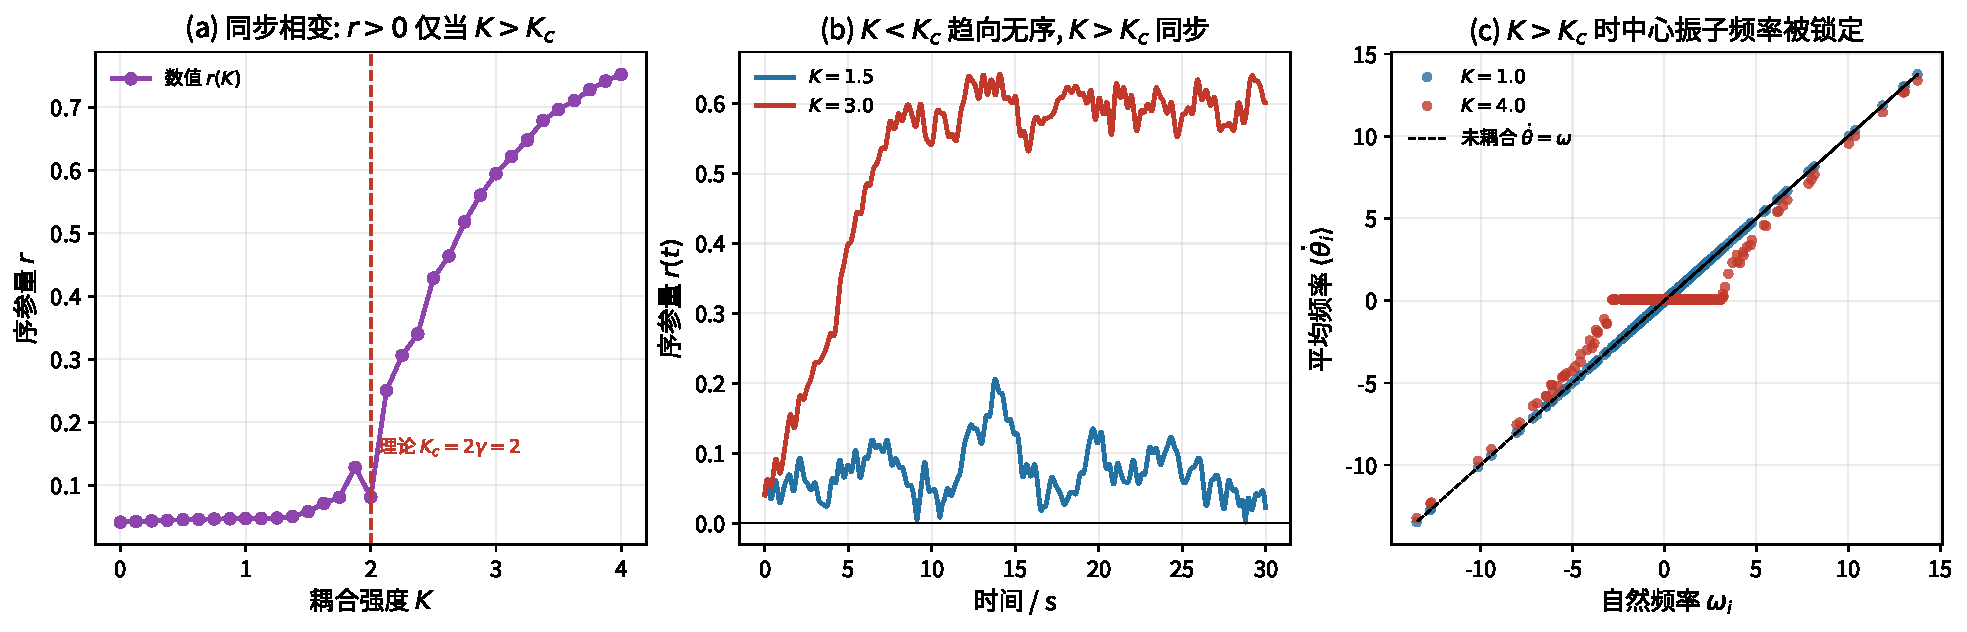
\includegraphics[width=0.99\textwidth]{fig11_kuramoto_transition.pdf}
\caption{\textbf{这张图说明}：耦合要强到什么程度，整个网络才会同步。
\textbf{画的是什么}：(a) 稳态序参量 $r$（$r=0$ 为无序、$r=1$ 为完全同步）与耦合强度 $K$ 的关系（带点线），
红色竖虚线为理论值 $K_c=2\gamma$（$\gamma$ 为自然频率分布 $g(\omega)$ 的 Lorentzian 半宽，本例 $\gamma=1$，故 $K_c=2$）。
(b) 两种耦合强度下 $r$ 随时间的演化 $r(t)$。
(c) 各振子的平均频率 $\langle\dot\theta_i\rangle$ 与自然频率 $\omega_i$ 的关系，黑虚线为未耦合情形 $\dot\theta=\omega$。
振子数 $N=400$。
\textbf{怎么读}：(a) $r$ 在 $K_c$ 处由零转为正，即同步相变；(c) $K>K_c$ 时中部一段振子的频率被锁定（水平段），边缘振子仍漂移。
\textbf{直观理解}：耦合太弱时，每个振子按自己的频率转，谁也带不动谁；
耦合超过一个门槛后，中间的振子被“拉住”、频率趋于一致——这个门槛就是 $K_c$。
门槛高低取决于“大家频率差得有多大”（分布越宽越难同步）。
\textbf{结论}：临界耦合有解析式 $K_c=2/(\pi g(0))$，可作为宏观同步性指标。}
\label{fig:transition}
\end{figure}

电网映射：$K_c$ 越大表示需要越强的网架/越大的耦合才能维持同步；
这为“承载力”提供了一个\textbf{宏观同步性指标}（序参量 $r$）的建模思路。
但必须注意图~\ref{fig:grid} 的结论：拓扑稀疏时同步阈值显著提高，
全连接的式~\eqref{eq:Kc} 不能直接搬到电网。

\begin{figure}[htbp]
\centering
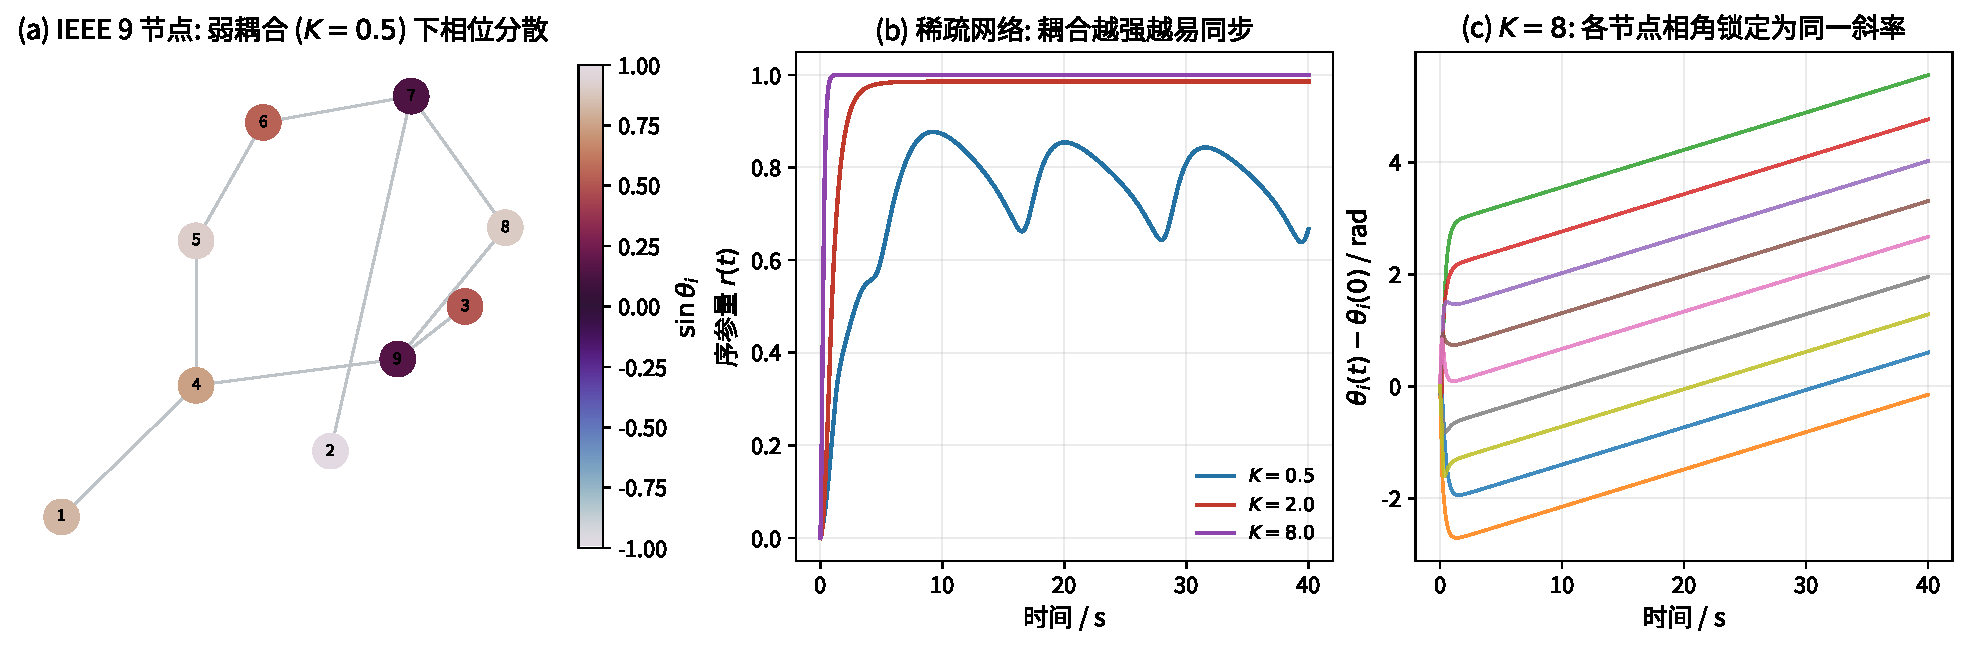
\includegraphics[width=0.99\textwidth]{fig12_kuramoto_grid.pdf}
\caption{\textbf{这张图说明}：在真实网络拓扑上，同步是更容易还是更难。
\textbf{画的是什么}：(a) IEEE 9 节点拓扑，节点颜色按 $\sin\theta_i$ 着色（$\theta_i$ 为节点相角），此例取弱耦合 $K=0.5$。
(b) 三种耦合强度下序参量 $r(t)$ 的演化。
(c) $K=8$ 时各节点相角（减去各自初值）随时间的演化。
\textbf{怎么读}：(a) 颜色分散表示相位分散；(b) 耦合越强 $r$ 越大、越早趋稳；(c) 强耦合时所有曲线合成一根斜线，即相角被锁定。
\textbf{为什么}：耦合项沿网络的边累加，稀疏网络中每个节点只与少数邻居相连，
有效耦合更弱，因此必须用更大的 $K$ 才能达到同样的同步程度；
这也是全连接公式 $K_c=2/(\pi g(0))$ 不能直接外推的原因。
\textbf{直观理解}：耦合是沿着边“传递”的——邻居越少，每个振子受到的拉力越弱，
所以要更大的 $K$ 才能把它们拉成同步。
\textbf{结论}：拓扑稀疏时同步更难，全连接的 $K_c$ 公式不能直接搬到真实网络。}
\label{fig:grid}
\end{figure}

\paragraph{小问题：$K_c=2\gamma$ 对电网意味着什么？}
$\gamma$ 是节点有功不平衡（自然频率）分布的离散程度，$K_c$ 是维持同步所需的
最小耦合强度。映射到电网：
$K_c$ 越大，说明需要越强的网架（$B_{ij}=1/X_{ij}$ 越大）或越小的不平衡才能同步。
于是“接入更多 DER”在 Kuramoto 语言里等价于“$\gamma$ 增大而 $K_c$ 不变”，
结果是同步裕度下降。


\subsection{与 RMS 的关系：降阶，而非等价}

综合 \S\ref{sec:singular} 与本节推导，四类模型之间是一个\textbf{简化关系}——注意其中
PF 与 Kuramoto 是两条并列的分支，而不是前后两级：

\begin{equation}
\begin{array}{rcl}
\text{EMT} & \xrightarrow[\text{平均开关}]{\text{忽略网络电磁暂态}} & \text{RMS}\\[5pt]
\text{RMS} & \xrightarrow[\text{令所有导数}=0]{\ \ \text{静态化}\ \ } & \text{PF / QSTS}\\[5pt]
\text{RMS} & \xrightarrow[\text{恒幅值、无损纯感}]{\text{相角化（消去网络）}} & \text{Kuramoto}
\end{array}
\label{eq:chain}
\end{equation}
\textbf{读法}：前两行是一条链（EMT $\to$ RMS）；后两行是 RMS 的\textbf{两个并列简化}——
PF 丢掉时间维度（静态化），Kuramoto 保留时间但消去网络与电压（相角化）。
因此 Kuramoto \textbf{不是}“潮流的进一步简化”：它比 PF 保留了转子摇摆动态，
只是把状态从“电压 $+$ 相角”压缩到“仅相角”。
表~\ref{tab:kuramoto-rms} 给出 Kuramoto 与 RMS 的逐项对照。

\begin{table}[htbp]
\centering
\caption{Kuramoto 与 RMS 的关系}
\label{tab:kuramoto-rms}
\small
\begin{tabularx}{\textwidth}{@{}lXX@{}}
\toprule
 & \textbf{RMS} & \textbf{Kuramoto} \\
\midrule
状态变量 & $\delta,\omega,E_q',E_d'$, 控制器状态 & 仅 $\delta_i$（一阶）或 $\delta_i,\omega_i$（二阶） \\
电压幅值 & 变量（$V_i$ 动态由网络/励磁决定） & 常数 $V_i\equiv V$（假设 A2） \\
网络 & 代数约束式~\eqref{eq:power-flow}，含 $G_{ij},B_{ij}$ & 直接消去为 $\sin$ 耦合，仅 $B_{ij}$（假设 A1） \\
无功/损耗 & 保留 & 全部丢弃 \\
可解析性 & 一般需数值积分 & 有相变等解析结论（式~\eqref{eq:Kc}） \\
适用场景 & 通用（输电/配电、弱网） & $X/R\gg1$、强电压支撑、宏观同步问题 \\
\bottomrule
\end{tabularx}
\end{table}

\paragraph{结论。}
Kuramoto 是 RMS 在三个强假设下的\textbf{降阶模型}，不是等价模型：
\begin{enumerate}[leftmargin=1.6em]
\item 在高压输电网（$X/R\sim5\text{--}20$、电压支撑强）的\textbf{同步稳定性}问题上，
它保留了主要机制，可作为解析工具（相变、临界耦合）；
\item 在配电网（$R/X\sim1\text{--}5$）和以电压问题为主导的场景中，
假设 A1--A2 均不成立（图~\ref{fig:swing}c 已量化 $R/X$ 的影响），
Kuramoto 只能做定性/宏观指标，不能替代潮流或 RMS；
\item 对本项目，Kuramoto 的价值在于为“城市电网承载力的宏观同步性判据”
提供一个\textbf{可解析、可解释}的骨架，但必须同时报告其假设边界。
此外，变流器下垂控制（droop control）与 Kuramoto 已有严格对应\cite{simpsonporco2013}，
可作为 DER 占比进一步提高后的扩展方向。
\end{enumerate}

\paragraph{小问题：Kuramoto 与 RMS 是等价、近似还是降阶？配电网能用吗？}
是\textbf{降阶}（reduction）而非等价：丢掉了电压幅值动态、无功与网络损耗，
逐项对照见表~\ref{tab:kuramoto-rms}。
配电网（$R/X\sim1$--$5$）中假设 A1 直接失效，且配电网的核心问题通常是
电压越限与三相不平衡而非功角同步，因此 Kuramoto 只能用作定性/宏观指标，
不能替代潮流或 RMS；这一点由图~\ref{fig:swing}(c) 的 $R/X$ 扫描直接量化。

\begin{figure}[htbp]
\centering
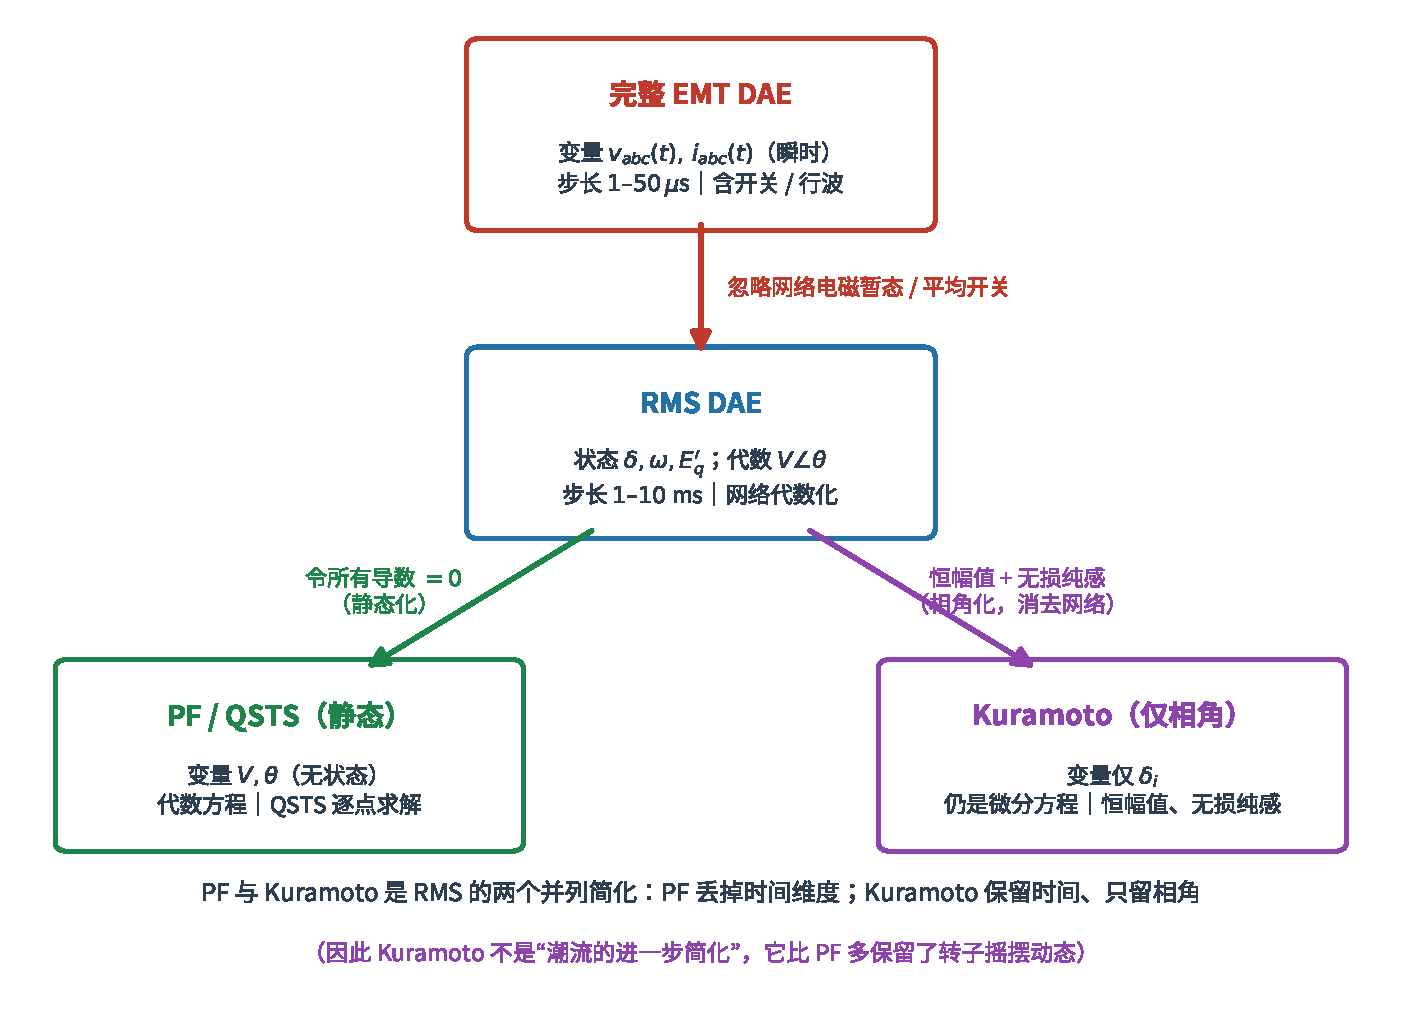
\includegraphics[width=0.99\textwidth]{fig13_model_chain.pdf}
\caption{\textbf{这张图说明}：这几类模型到底是什么关系（是本报告的总览图）。
\textbf{看图}：四列方框依次为完整 EMT、RMS、潮流/功率平衡、Kuramoto；
框间箭头标注各次降阶丢掉的动态，下方灰框标注代价或损失。
\textbf{为什么}：PF 是“令所有导数为零”（丢掉时间维度）；Kuramoto 是“保留时间、但用恒幅值 $+$ 无损
把网络代数约束解析消去”（丢掉电压与网络）。两者丢掉的量不同，因此是并列而非前后两级。
\textbf{直观理解}：PF 是把“时间”整个丢掉（只看稳态）；Kuramoto 是保留时间、但把“电压与网络”丢掉。
两者丢掉的不是同一样东西，所以是并列的两条路，而不是前后两级。
\textbf{结论}：EMT、RMS、PF 是一条链，而 Kuramoto 是 RMS 的\textbf{并列简化}（不是链上下一级）；
Q3 回答前两级的连接，Q4 回答 Kuramoto 从哪来、代价是什么。}
\label{fig:chain}
\end{figure}

\section{小结与对项目下一步的建议}
\label{sec:summary}

\subsection{假设与适用条件汇总}

本报告的每个定量结论都依赖明确的假设。为便于核查与质疑，
表~\ref{tab:assumptions} 汇总“结论--假设--失效条件”，避免把某条结论
误用到其假设不成立的场景。

\begin{table}[htbp]
\centering
\caption{主要结论所依赖的假设与失效条件}
\label{tab:assumptions}
\small
\begin{tabularx}{\textwidth}{@{}lXX@{}}
\toprule
结论 & 依赖的假设 & 失效条件 \\
\midrule
潮流方程（式~\eqref{eq:power-flow}） & 稳态、单一频率、输电网三相平衡 &
频率显著偏离、三相不平衡（配电网需三相 PF） \\
RMS 可代数化网络（式~\eqref{eq:rms-dae}） & 网络电磁暂态远快于机电动态 &
变流器带宽接近网络谐振频率 \\
准稳态误差（式~\eqref{eq:qs-error}） & 包络带宽 $\Omega\ll\omega_s$ &
$\Omega/\omega_s$ 或调制深度 $m$ 大 \\
奇异摄动降阶（式~\eqref{eq:slow-manifold}） & 快子系统一致渐近稳定、$\varepsilon\ll1$ &
快子系统失稳，或 $\varepsilon$ 不够小 \\
混合接口（式~\eqref{eq:delay-error}、\eqref{eq:nyquist}） &
功率按周期平均守恒、延迟小、满足采样定理 & 高次谐波显著、延迟接近半周期 \\
Kuramoto（式~\eqref{eq:swing-kuramoto}） &
(A1) 无损、(A2) 恒幅值、(A3) 均匀惯性/过阻尼 & $R/X$ 不小、电压问题主导 \\
\bottomrule
\end{tabularx}
\end{table}

\subsection{五条核心结论}

\begin{enumerate}[leftmargin=1.8em]
\item \textbf{三类模型的差别是“保留哪些动力学”，不是“精度高低”。}
同一电网的现象跨越约 15 个数量级（图~\ref{fig:timescales}），
PF/QSTS、RMS、EMT 各覆盖一段，逐条保留/忽略清单见表~\ref{tab:retention}。
\item \textbf{潮流与 RMS 的连接有两层含义}：
工作点层（潮流 $=$ RMS 的平衡点，传 $V\angle\theta$ 与 $P,Q$，\S\ref{sec:workpoint}）
与瞬时--相量层（EMT 与 RMS 交换三相瞬时值与基频相量，\S\ref{sec:phasor-link}）。
\item \textbf{降阶是否安全有可计算的判据}：
准稳态误差 $\varepsilon=m(\Omega/\omega_s)\sin\phi_z$（式~\eqref{eq:qs-error}），
其数学本质是奇异摄动的慢流形极限（式~\eqref{eq:slow-manifold}），
工程上表现为刚度比 $10^4$--$10^6$（图~\ref{fig:spectrum}）。
\item \textbf{混合仿真的接口有两条硬约束}：
Nyquist（$\Delta t_r<1/(2f_h)$）与延迟误差（$\approx\omega_s\tau\cot\theta$），
二者共同决定了 RMS 侧在混合仿真中也必须用小步长（图~\ref{fig:interface}）。
\item \textbf{Kuramoto 是 RMS 的降阶模型}，其成立依赖三个强假设
（无损、恒幅值、均匀惯性/过阻尼）；在输电网同步问题中可用且有相变等解析结论，
在配电网（$R/X$ 大、电压主导）不可替代潮流/RMS（图~\ref{fig:swing}--\ref{fig:chain}）。
\end{enumerate}

\subsection{与项目书技术点/难点的对应}

\begin{itemize}[leftmargin=1.6em]
\item \textbf{技术内容第一点}（分布式资源高维非线性接入行为建模）：
本报告给出 DER 接入后“在哪个时间尺度建模、用什么模型”的选择依据（\S\ref{sec:q2}）。
\item \textbf{技术内容第二点}（有限元/伽辽金改进潮流计算）：
给出“潮流作为降阶目标”的误差判据（式~\eqref{eq:qs-error}、式~\eqref{eq:eps-grid}），
为降阶加速设定可接受的误差上界。
\item \textbf{技术难点第二点}（多源不确定性难刻画）：
说明不确定性在不同尺度上的表现不同——快尺度是随机开关/纹波，
慢尺度是出力时序，二者需用不同模型（QSTS 场景法 vs EMT 波形统计）。
\item \textbf{专利 1（电网建模，以 DER 建模为重点）}：
可直接引用“三模型保留矩阵（表~\ref{tab:retention}）+ 接口变量定义（图~\ref{fig:hybrid}）”
作为权利要求中“模型选择/切换条件”的技术依据。
\end{itemize}

\subsection{对第二次讨论的准备建议}

\begin{enumerate}[leftmargin=1.6em]
\item \textbf{数据与 benchmark}：建议至少准备
（i）一个输电网测试系统（IEEE 9/39）用于 RMS 与 Kuramoto 对照；
（ii）一个配电网测试系统（IEEE 34/123 节点）用于三相不平衡 PF/QSTS；
（iii）DER 时序数据（光伏/负荷/EV），用于 QSTS。
本报告的图已用到 IEEE 9 节点拓扑（图~\ref{fig:grid}），可直接复用。
\item \textbf{建模框架}：建议以“潮流为骨架 $+$ DER 时序模块 $+$ 不确定性场景生成”
作为主线框架；RMS/EMT 作为校验模块，Kuramoto 作为指标模块。
与式~\eqref{eq:chain} 的链条一一对应。
\item \textbf{待确认的问题（需项目组讨论）}：
（i）承载力指标的“动态”程度——是纯 QSTS 越限统计，还是要含机电暂态裕度？
（ii）是否允许把 Kuramoto 的序参量 $r$ 作为承载力的一项输出指标？
（iii）配电网三相不平衡是否必须显式建模（决定用 DistFlow 还是三相 PF）。
\end{enumerate}

\subsection{边界与开放问题}

本报告的每条结论都带有明确的使用边界（表~\ref{tab:assumptions}）。
这些边界主要不是“尚未完成的工作”，而是跨尺度降阶本身的性质：降阶必然伴随信息损失。
由此可提出三个可继续深入的问题：

\begin{enumerate}[leftmargin=1.6em]
\item \textbf{数据驱动的慢流形}：能否不经解析推导，直接从 EMT 仿真数据中学出
RMS 的慢流形表示？（对应“用机器学习做复杂系统降阶”的思路。）
\item \textbf{误差判据的推广}：式~\eqref{eq:qs-error} 的误差界能否直接用作学习型
代理模型（surrogate model）的验收标准——即“误差低于该界，才允许用代理模型替代动态仿真”？
\item \textbf{配电网的降阶指标}：当 $R/X$ 不小、假设 (A1) 失效时，
是否存在替代 Kuramoto、但仍可解析的降阶指标？
\end{enumerate}

其余技术性限制（例如图~\ref{fig:spectrum} 的特征值算例为 $10$ 阶简化系统、
混合仿真的稳定性只给出两条约束）已在正文相应位置随结论说明，不在此重复。

\section{图表与脚本索引}
\label{sec:index}

表~\ref{tab:index} 汇总“问题--图--脚本--结论”：每张图由哪个脚本生成、回答哪个问题、一句话结论是什么。
全部图由 \texttt{python/} 下脚本现场数值计算，参数写在脚本内，关键数值存于 \texttt{data/*.npz}；
矢量版为 \texttt{figures/*.pdf}（供 LaTeX 引用），位图版为 \texttt{figures/*.png}。

\begin{table}[htbp]
\centering
\caption{问题--图--脚本索引}
\label{tab:index}
\small
\begin{tabularx}{\textwidth}{@{}lllX@{}}
\toprule
问题 & 图/表 & 脚本 & 该图要说明的一句话结论 \\
\midrule
Q1 & \ref{fig:timescales} & \texttt{fig01\_timescales.py} & 同一电网的现象跨越 15 个数量级，三类模型各覆盖一段 \\
Q1 & 表~\ref{tab:retention} & \texttt{fig02\_assumptions.py} & 三模型对每个物理过程保留/近似/忽略的完整清单 \\
Q3 & \ref{fig:park} & \texttt{fig03\_park.py} & 平衡正序时 dq 为直流；不平衡出现 $2\omega$ 纹波，相量法失效 \\
Q3 & \ref{fig:phasor} & \texttt{fig04\_phasor.py} & 相量法丢掉的暂态严格按 $e^{-t/\tau}$ 衰减，最坏合闸时与稳态同量级 \\
Q3 & \ref{fig:quasistatic} & \texttt{fig05\_quasistatic.py} & 准稳态误差 $\approx m(\Omega/\omega)\sin\phi_z$：判据是包络带宽 $\ll$ 载波频率 \\
Q3 & \ref{fig:singular} & \texttt{fig06\_singular.py} & RMS 是 EMT 在 $\varepsilon\to0$ 的慢流形极限，快动态只存在于 $O(\varepsilon)$ 边界层 \\
Q3 & \ref{fig:spectrum} & \texttt{fig07\_spectrum.py} & 线性化系统特征值分成两团，刚度比 $\sim10^4$，这是全阶仿真的根本困难 \\
Q3 & \ref{fig:hybrid} & \texttt{fig08\_hybrid.py} & 混合仿真的接口交换“瞬时波形$\leftrightarrow$基频相量”，代价是延迟与插值误差 \\
Q3 & \ref{fig:interface} & \texttt{fig09\_interface.py} & 接口误差的两条硬约束：Nyquist 混叠与 $\omega\tau\cot\theta$ 延迟误差 \\
Q4 & \ref{fig:swing} & \texttt{fig10\_swing\_kuramoto.py} & swing 方程在无损纯感、恒幅值假设下即为 Kuramoto 模型 \\
Q4 & \ref{fig:transition} & \texttt{fig11\_kuramoto\_transition.py} & 耦合增强时出现同步相变，临界耦合有解析解 \\
Q4 & \ref{fig:grid} & \texttt{fig12\_kuramoto\_grid.py} & 真实网络拓扑上的 Kuramoto 同步过程与序参量演化 \\
Q4 & \ref{fig:chain} & \texttt{fig13\_model\_chain.py} & 完整 DAE $\to$ RMS $\to$ Kuramoto 的近似链条与信息损失 \\
\bottomrule
\end{tabularx}
\end{table}

\paragraph{小问题：这些图是“自己算的”还是“找来的”？}
全部由 \texttt{python/} 下脚本现场数值计算生成，可重复运行；
每张图的坐标轴含义、参数取值、解析对照都在正文首次引用处给出，
关键数值另存 \texttt{data/*.npz}。如需复核某个数值，可直接打开对应脚本与数据文件。

\appendix

\section{从 KCL 到潮流方程（完整推导）}
\label{app:powerflow}

本附录给出正文式~\eqref{eq:power-flow} 的完整推导，供查阅；
正文只引用结论（该推导属项目第 1 项“潮流/QSTS”任务的调研范围）。

设网络有 $n$ 个节点，节点注入电流与节点电压的关系由基尔霍夫电流定律给出：
\begin{equation}
\bI=\bY\bV,\qquad \bY=\bG+\jj\bB ,
\label{eq:app-kcl}
\end{equation}
其中节点导纳矩阵由支路导纳 $y_{km}=1/(R_{km}+\jj X_{km})$ 与对地支路组装：
\begin{equation}
Y_{ik}=
\begin{cases}
\displaystyle\sum_{m\in\mathcal{N}(i)}\!\!\Bigl(g_{im}+\jj b_{im}\Bigr)+y_{i0}, & i=k,\\[6pt]
-\bigl(g_{ik}+\jj b_{ik}\bigr), & i\neq k,\ i\sim k,\\[2pt]
0, & \text{否则}.
\end{cases}
\label{eq:app-ybus}
\end{equation}
节点 $i$ 的复功率为 $S_i=V_iI_i^{*}$；把式~\eqref{eq:app-kcl} 代入并取共轭：
\begin{equation}
S_i=V_i\sum_{k=1}^{n}Y_{ik}^{*}V_k^{*}.
\label{eq:app-scomplex}
\end{equation}
写 $V_i=V_ie^{\jj\theta_i}$、$Y_{ik}=G_{ik}+\jj B_{ik}$、$\theta_{ik}=\theta_i-\theta_k$，
分离实部与虚部即得式~\eqref{eq:power-flow}。按已知量分类：
PQ 节点给定 $P_i,Q_i$，PV 节点给定 $P_i,V_i$，平衡节点给定 $V,\theta$；
式~\eqref{eq:power-flow} 为 $2n$ 个代数方程，用牛顿--拉夫逊法求解，
雅可比矩阵 $\partial(P,Q)/\partial(\theta,V)$ 具有式~\eqref{eq:app-ybus} 的稀疏结构，
在解附近二阶收敛（典型 $3$--$5$ 次迭代）。

\section{RL 支路 $dq$ 方程的完整推导}
\label{app:rldq}

正文推导块 2 给出的结论式~\eqref{eq:rl-dq} 推自 $abc$ 域方程。由
\begin{equation}
\bm{v}_{abc}=R\,\bm{i}_{abc}+L\,\frac{\dd\bm{i}_{abc}}{\dd t},
\qquad \bm{i}_{abc}=\bT^{-1}(\theta)\bm{i}_{dq0},
\end{equation}
代入并注意 ${\dd\bT^{-1}}/{\dd t}=\bT^{-1}\dot\theta\,\bm{S}$（$\bm S$ 为 $90^\circ$ 旋转），得
\begin{equation}
\bm{v}_{dq0}=R\,\bm{i}_{dq0}+L\,\bT^{-1}\frac{\dd\bm{i}_{dq0}}{\dd t}
+L\,\bT^{-1}\dot\theta\,\bm{S}\,\bm{i}_{dq0}.
\end{equation}
左乘 $\bT$（即得到 $dq0$ 分量）并令 $\dot\theta=\omega$，即得
\begin{equation}
v_d=R\,i_d+L\,\dif{i_d}{t}-\omega L\,i_q,\qquad
v_q=R\,i_q+L\,\dif{i_q}{t}+\omega L\,i_d .
\end{equation}
其中 $\omega L$ 项来自坐标旋转（非电磁暂态），$L\,\dd i/\dd t$ 项才是电磁暂态。

\section{软件与 benchmark 清单}
\label{app:tools}

\begin{table}[H]
\centering
\caption{三类模型的常用软件与测试系统}
\label{tab:tools}
\small
\begin{tabularx}{\textwidth}{@{}lXX@{}}
\toprule
 & 常用软件 & 常用测试系统 / 数据 \\
\midrule
PF / QSTS & MATPOWER、pandapower、OpenDSS、PSS\textsuperscript{\textregistered}E、PowerFactory &
IEEE 9/14/30/39/118；IEEE 13/34/123 馈线；CIGRE MV/LV \\
RMS & PSS\textsuperscript{\textregistered}E、PowerFactory、Dynawo、ANDES &
WSCC 3 机 9 节点；IEEE 双区域 4 机；Nordic 32 机 \\
EMT & PSCAD/EMTDC、EMTP-RV、ATP、Simscape Electrical &
IEEE 9 节点 EMT 算例；CIGRE B4 直流基准；WECC 第二基准 \\
\bottomrule
\end{tabularx}
\end{table}

数据来源建议：网络参数取 MATPOWER 算例与 IEEE PES 测试馈线文档；
光伏/风电出力取 NREL 公开数据集；负荷曲线取 IEEE 测试馈线负荷与 OpenEI；
EV 充电取公开充电站数据集。注意时间分辨率须与模型匹配：
QSTS 用 $1$--$15$ min，EMT 用 $\mu$s 级波形，二者不可混用。

\section{缩略语表}
\label{app:abbr}

\begin{table}[H]
\centering
\small
\begin{tabularx}{\textwidth}{@{}l l X@{}}
\toprule
缩写 & 英文全称 & 中文含义 \\
\midrule
EMT & Electromagnetic Transient & 电磁暂态（直接求解瞬时量的模型） \\
RMS & Root-Mean-Square & 机电暂态/相量域动态仿真（本文取此义） \\
PF & Power Flow & 潮流 \\
QSTS & Quasi-Static Time-Series & 准稳态时序 \\
DAE & Differential-Algebraic Equation & 微分--代数方程 \\
DER & Distributed Energy Resource & 分布式能源（光伏、储能、电动汽车等） \\
IBR & Inverter-Based Resource & 变流器型电源（经变流器接入的电源） \\
VSC & Voltage Source Converter & 电压源型变流器 \\
GFL / GFM & Grid-Following / Grid-Forming & 跟网型 / 构网型变流器控制 \\
PLL & Phase-Locked Loop & 锁相环 \\
PWM & Pulse Width Modulation & 脉宽调制 \\
DFT & Discrete Fourier Transform & 离散傅里叶变换（本文用于相量提取） \\
PSS & Power System Stabilizer & 电力系统稳定器（抑制低频振荡） \\
CDA & Critical Damping Adjustment & 临界阻尼调整（EMT 数值方法） \\
\bottomrule
\end{tabularx}
\end{table}

\section{主要符号表}
\label{app:symbols}

供读者忘记符号时查阅；正文中每个符号首次出现处均给出定义。
下表按“通用 $\to$ 网络与潮流 $\to$ EMT 与数值方法 $\to$ 动态/降阶/接口 $\to$ Kuramoto”分组。

\begin{longtable}{@{}l p{7.4cm} l@{}}
\caption{主要符号表（按类别分组）}\label{tab:symbols}\\
\toprule
符号 & 含义 & 首次出现 \\
\midrule
\endfirsthead
\toprule
符号 & 含义 & 首次出现 \\
\midrule
\endhead
\bottomrule
\endlastfoot
\multicolumn{3}{@{}l}{\textbf{（1）通用}}\\
$n$ & 节点（或振子）数目 & \S\ref{sec:q2} \\
$t$ & 时间 & 式~\eqref{eq:emt-dae} \\
$\jj$ & 虚数单位 & 式~\eqref{eq:power-flow} \\
$\Real\{\cdot\},\ \Imag\{\cdot\}$ & 取实部、取虚部 & 式~\eqref{eq:kuramoto-meanfield} \\
$\omega_s$ & 同步角频率（$2\pi\times50$ rad/s） & \S\ref{sec:phasor-link} \\
$T$ & 工频周期（$20$ ms） & 式~\eqref{eq:power-consistency} \\
$\bm{x}$ & 状态变量（需初值、随时间演化） & 式~\eqref{eq:emt-dae} \\
$\bm{y}$ & 代数变量（由约束即时确定） & 式~\eqref{eq:rms-dae} \\
$\bm{z}$ & 快变量（电磁暂态量） & 式~\eqref{eq:singular} \\
$\bm{u}$ & 输入/控制变量（$P_m$、励磁、变流器指令） & 式~\eqref{eq:emt-dae} \\
$\bm{f},\ \bm{g}$ & 微分方程右端、代数约束函数 & 式~\eqref{eq:emt-dae} \\
\midrule
\multicolumn{3}{@{}l}{\textbf{（2）网络与潮流}}\\
$V_i,\ \theta_i$ & 节点 $i$ 的电压幅值与相角 & 式~\eqref{eq:power-flow} \\
$P_i,\ Q_i$ & 节点 $i$ 的注入有功、无功 & 式~\eqref{eq:power-flow} \\
$S_i=P_i+\jj Q_i$ & 节点 $i$ 的复功率 & 式~\eqref{eq:power-flow} \\
$\theta_{ik}$ & 相角差 $\theta_i-\theta_k$ & 式~\eqref{eq:power-flow} \\
$G_{ik},\ B_{ik}$ & 节点导纳矩阵元素的实部、虚部 & 式~\eqref{eq:power-flow} \\
$\bm{Y},\ \bm{G},\ \bm{B}$ & 节点导纳矩阵及其实部、虚部 & 式~\eqref{eq:app-kcl} \\
$y_{km},\ g_{km},\ b_{km}$ & 支路导纳及其实部、虚部 & 式~\eqref{eq:app-ybus} \\
$R_{ik},\ X_{ik}$ & 支路电阻、电抗 & 式~\eqref{eq:app-ybus} \\
$H$ & 同步机惯性时间常数（$2$--$9$ s） & \S\ref{sec:q1} \\
$\bm{T}(\theta)$ & Park 变换矩阵 & 式~\eqref{eq:park} \\
$\bm{S}$ & $90^\circ$ 旋转矩阵 & 附录~\ref{app:rldq} \\
\midrule
\multicolumn{3}{@{}l}{\textbf{（3）EMT 与数值方法}}\\
$L,\ C,\ R$ & 电感、电容、电阻 & 式~\eqref{eq:emt-elements} \\
$i_L,\ v_C$ & 电感电流、电容电压 & 式~\eqref{eq:emt-elements} \\
$Z_c,\ \tau$ & 行波波阻抗、行波穿越时间 & \S\ref{sec:q1} \\
$\Delta t$ & 积分步长（下标 $e$ 为 EMT、$r$ 为 RMS） & 式~\eqref{eq:emt-dt} \\
$f_{\max}$ & 最高关心频率（决定 EMT 步长） & 式~\eqref{eq:emt-dt} \\
$N$ & 步长比 $\Delta t_r/\Delta t_e$ & \S\ref{sec:hybrid} \\
\midrule
\multicolumn{3}{@{}l}{\textbf{（4）动态、降阶与接口}}\\
$\delta_i,\ \omega_i$ & 转子角、转速（偏差） & 式~\eqref{eq:swing} \\
$E_q'$ & $q$ 轴暂态电势 & \S\ref{sec:q2} \\
$M_i,\ D_i$ & 惯性常数、阻尼系数 & 式~\eqref{eq:swing} \\
$P_{m,i},\ P_{e,i}$ & 机械功率、电磁功率 & 式~\eqref{eq:swing} \\
$\varepsilon$ & 快慢时间常数之比（$10^{-4}$--$10^{-6}$） & 式~\eqref{eq:singular} \\
$\bm{h}(\bm{x})$ & 慢流形映射（快变量由慢变量决定） & 式~\eqref{eq:slow-manifold} \\
$\bm{f}_r$ & 降阶后的右端函数 & 式~\eqref{eq:slow-manifold} \\
$\lambda_i,\ \kappa$ & 特征值、刚度比 & \S\ref{sec:eigen} \\
$Z(\jmath\omega_s)=R+\jj\omega_sL$ & 支路阻抗 & 式~\eqref{eq:quasi-static} \\
$\phi_z$ & 阻抗角 $\arctan(\omega_sL/R)$ & 式~\eqref{eq:qs-error} \\
$m,\ \Omega$ & 包络调制深度、包络带宽 & 式~\eqref{eq:qs-error} \\
$V(t),\ I(t)$ & 电压、电流的复包络 & 式~\eqref{eq:envelope-ode} \\
$I_0,\ \delta I$ & 零阶（相量）解、一阶修正 & 式~\eqref{eq:quasi-static} \\
$\tau_d$ & 接口延迟 & 式~\eqref{eq:delay-error} \\
$Y_n,\ I_n$ & 诺顿等值导纳、电流源 & \S\ref{sec:hybrid} \\
$E_{th},\ Z_{th}$ & 戴维南等值电压源、阻抗 & \S\ref{sec:hybrid} \\
$f_h$ & EMT 侧最高关心谐波频率 & 式~\eqref{eq:nyquist} \\
\midrule
\multicolumn{3}{@{}l}{\textbf{（5）Kuramoto 模型}}\\
$\theta_i$（振子） & 振子相位（对应电网相角 $\delta_i$） & 式~\eqref{eq:kuramoto} \\
$\omega_i$（振子） & 自然频率（对应有功不平衡） & 式~\eqref{eq:kuramoto} \\
$K,\ K_{ij}$ & 耦合强度（$K_{ij}=V_iV_jB_{ij}$） & 式~\eqref{eq:swing-kuramoto} \\
$r$ & 序参量（$0$ 无序，$1$ 完全同步） & 式~\eqref{eq:order-param} \\
$\psi$ & 序参量的平均相位 & 式~\eqref{eq:order-param} \\
$g(\omega)$ & 自然频率分布 & 式~\eqref{eq:Kc} \\
$\gamma$ & Lorentzian 分布的半宽 & \S\ref{sec:q4} \\
$\delta(\cdot)$ & Dirac $\delta$ 函数 & 式~\eqref{eq:selfconsistent} \\
\end{longtable}

\section{关键设备与概念的简要说明}
\label{app:concepts}

面向不熟悉电力系统的读者；每条一到两句，按“设备 $\to$ 控制 $\to$ 建模用语”排列。

\begin{table}[H]
\centering
\small
\renewcommand{\arraystretch}{1.12}
\begin{tabularx}{\textwidth}{@{}lX@{}}
\toprule
概念 & 简要说明 \\
\midrule
同步机 & 与电网同频率旋转的发电机（火电、水电、核电主力机型）；
提供惯量，是传统电网动态的核心。 \\
转子角 $\delta$、转速 $\omega$ & 转子相对同步旋转参考系的角位置与角速度；
$\delta$ 超出稳定边界即“失步”。 \\
惯性常数 $M$（或 $H$） & 转子转动惯量折算到电气量；$M$ 越大频率变化越慢。 \\
阻尼系数 $D$ & 抑制转子振荡的等效阻尼（机械与电气部分之和）。 \\
励磁系统 / AVR & 调节励磁电流以维持发电机端电压；时间常数约 $0.1$ 秒至数秒。 \\
调速器 / 原动机 & 按频率偏差调整机械功率；时间常数数秒至数十秒。 \\
PSS & 电力系统稳定器：附加励磁控制，抑制低频振荡。 \\
变流器（VSC/逆变器） & 电力电子开关装置，把直流变换为交流；控制灵活但没有固有惯量。 \\
IBR / DER & 经变流器接入的电源（光伏、风电、储能、电动汽车）；
IBR（Inverter-Based Resource）强调“经变流器接入”。 \\
GFL / GFM & 跟网型（跟随电网相位、需锁相环）／构网型（自建电压与频率、可支撑惯量）。 \\
PLL & 锁相环：跟网型变流器用来测量电网相位的环节，其动态是 EMT 关注的快动态之一。 \\
内环 / 外环控制 & 内环控电流（千赫兹级，快）、外环控功率或电压（较慢）；
两者保留程度不同，正是 EMT 与 RMS 的差别之一。 \\
载波 / 包络 & 载波指 $50$ Hz 工频正弦；包络指其幅值随时间的慢变轮廓。 \\
准稳态 & 假设包络变化足够慢、从而忽略其导数的近似（判据见式~\eqref{eq:qs-error}）。 \\
\bottomrule
\end{tabularx}
\end{table}


\small
\bibliographystyle{unsrt}
\bibliography{refs}

\end{document}
